\documentclass[12pt]{article}
\usepackage{geometry}
\geometry{left=1in,right=0.75in,top=1in,bottom=1in}

%%%%%%%%%%%%%%%%%%%%%%%%%%%%%%%%%%%%%%%%
% Replace ABCDEF in the next line with your chosen problem
% and replace 1111111 with your Team Control Number
\newcommand{\Problem}{D}
\newcommand{\Team}{2107714}
%%%%%%%%%%%%%%%%%%%%%%%%%%%%%%%%%%%%%%%%

\usepackage{newtxtext}
\usepackage{amsmath,amssymb,amsthm}


\usepackage[pdftex]{graphicx}
\usepackage{xcolor}
\usepackage{fancyhdr}
\usepackage{lastpage}
\usepackage{listings}

\usepackage{txfonts}    
\usepackage{indentfirst}
\usepackage{float}
\usepackage{graphicx}
\usepackage{subfigure} 
\usepackage{booktabs}


\lhead{Team \Team}
\rhead{}
\cfoot{}

\newtheorem{theorem}{Theorem}
\newtheorem{corollary}[theorem]{Corollary}
\newtheorem{lemma}[theorem]{Lemma}
\newtheorem{definition}{Definition}

%%%%%%%%%%%%%%%%%%%%%%%%%%%%%%%%
\begin{document}
\graphicspath{{.}}  % Place your graphic files in the same directory as your main document
\DeclareGraphicsExtensions{.pdf, .jpg, .tif, .png}
\thispagestyle{empty}
\vspace*{-16ex}
\centerline{\begin{tabular}{*3{c}}
	\parbox[t]{0.3\linewidth}{\begin{center}\textbf{Problem Chosen}\\ \Large \textcolor{red}{\Problem}\end{center}}
	& \parbox[t]{0.3\linewidth}{\begin{center}\textbf{2021\\ MCM/ICM\\ Summary Sheet}\end{center}}
	& \parbox[t]{0.3\linewidth}{\begin{center}\textbf{Team Control Number}\\ \Large \textcolor{red}{\Team}\end{center}}	\\
	\hline
\end{tabular}}
%%%%%%%%%%% Begin Summary %%%%%%%%%%%
% Enter your summary here replacing the (red) text
% Replace the text from here ...


~

\begin{center}
\Large\textbf{A Network Model for Music Influence, Similarity and Evolution}
\end{center}


~

%%%%%%%%         Summary begins here   %%%%%%%%
Music is developed under the mutual influence of artists from various genres. In the last ninety years, lots of great music has been created. We develop a network model based on some advanced algorithm to excavate the \textbf{significant evolutionary and revolutionary trends} of artists and genres. This paper is categorized into the main three-part, focusing on influence, similarity and evolution, for music genres and artists respectively.

~

Firstly, we process the data provided by the ICM Society. We sort out the number of followers and influencers with respect to artists and the music genres' basic information, which contains 14 main features. Then, we build a network model and analyze the modularity, density and average degree, which could represent the influence level of certain artists.
For the network model part, we get the rank of most influential artists from 1930 to 2010. The top 6 artists are: \emph{\textbf{The Beatles, Bob Dylan, The Rolling Stones, David Bowie, Led Zeppelin and Jimi Hendrix}}. All of them are Pop/Rock artists in 1960. Apart from that, we also get the top 1 most influential artist for each year and each genre separately. We find that the artists in the Pop/Rock genre are most influential and in the genre table, we can also get that the artists in 1960 are most influential, which is consistent with results get from the network diagram. The value of modularity greater than 0.44 indicates a certain degree of modularization had reached by the network diagram. We get 0.7030, 0.6950, 0.6180, 0.5260, 0.6060, 0.6570, 0.7180, 0.8990 and 0.9000 for each network diagram (in order of years from 1930 to 2010), which shows our network diagram is significant.

~

Next, we expand our model and establish a classification system by using a hierarchical clustering model to analyze the similarities and differences among those music genres. The highest correlation coefficient is 0.8473 for Pop/Rock and Religious. Moreover, the characteristic which could distinguish a genre is \textbf{speechiness}, since it has a low correlation with others characteristics. For a certain genre, the attraction must be focused on the \textbf{danceability, energy, valence, tempo and loudness}. Furthermore, combining with the network model, we consider the time and analyze the \textbf{evolution} processes of musical evolution and \textbf{revolution} that occurred over time in one genre.

~

Then, we could combine our quantitative analysis with the qualitative analysis by studying the literature background such as social, political, cultural and technological factors along with the music genres evolution. For instance, \textbf{regional immigration, Bop school, hippie youth movement, people's thoughts on war, economy}, the technological breakthrough of \textbf{music synthesizer} promote the development of Country, Jazz, R\&B and Pop/Rock, respectively. The key decade is the 1960s when \emph{The Beatles} dominated the music community. 

~

In the end, we write a report to ICM society about how we excavate the important value by our network model to help them understand our recommended further study of music and its effect on culture.

\textbf{Key Words:} Network model; Music Influence; Similarity; PCA; Hierarchical Clustering; Evolution


%%%%%%%%%%% End Summary %%%%%%%%%%%

%%%%%%%%%%%%%%%%%%%%%%%%%%%%%%

\clearpage
\pagestyle{fancy}
% Uncomment the next line to generate a Table of Contents
%\tableofcontents 
\newpage
\setcounter{page}{1}
\rhead{Page \thepage\ of \pageref{LastPage}}



\tableofcontents
\section{Introduction}
\subsection{Background}
Nowadays, music is a common thing around us, it can bring different emotions to people. Music is both the voice and memory of individuals and societies, providing a soundscape through which to listen and understand people, groups and their histories.

It is well established that there are many influences to artists when they composing music, including their natural creativity, current social or political events, the usage of a new musical instrument or tool, or other personal experiences. But how to evaluate the different influences of these things? It is necessary to consider the different results of these influences and develop mathematical models and methods to make a quantitative analysis.

\subsection{Restatement of the problem}
In order to evaluate the music influence among artists and genres, as well as the music revolution. We are required to answer the following questions.
\begin{enumerate}
    \item Create a (multiple) directed network(s) of musical influence to describe the musical influence and analyze what the musical influence the network(s) reveals.
    \item Develop a measure to explore music similarity and find out whether artists within the genre are more similar than artists between genres.
    \item Compare similarities and influences between different or the same genres. 
    \item Create a model to find out that whether the similarity data indicate the identified influencers in fact influence the respective artists.
    \item Find out whether there are characteristics in the network that can mark the revolution of music evolution and which artists represent the revolutionaries of the network created.
    \item Create a model to analyze the influence process of a genre's musical revolution over time. Indicate what reveal dynamic influencing factors is and explain how genres or artists have changed over time.
    \item Show that how does our work expresses the cultural influence of music in time or environment or Explain how to identify the impact of social, political or technological change within a network.
    
\end{enumerate}

\subsection{Overview of model}
Firstly, based on the data from the files given by ICM Society, we clean, select and standardize the data. More precisely, we sort out the number of followers and influencers with respect to artists and the music genres' basic information, which contains 14 main features. Secondly, we build a network model and analyze the \textbf{modularity, density and average degree}, which could represent the influence level of certain artists. Then by using the \textbf{principal component analysis skill}, we shift our focus to some main factors and build a similarity model based on cosine distance. Next, we expand our model and establish a classification system by using a \textbf{hierarchical clustering model} to analyze the similarities and differences among those music genres. Furthermore, combining with the network model, we consider the time and analyze the influence processes of musical evolution that occurred over time in one genre. Finally, after a lot of quantitative analysis, we introduce qualitative analysis techniques to conclude and summarize the model, factors like cultural, social, political or technological changes are taken into consideration.
The main framework of our model is showed as Figure \ref{overview}.
\begin{figure}[H]
\label{fig:aa}
\small
\centering
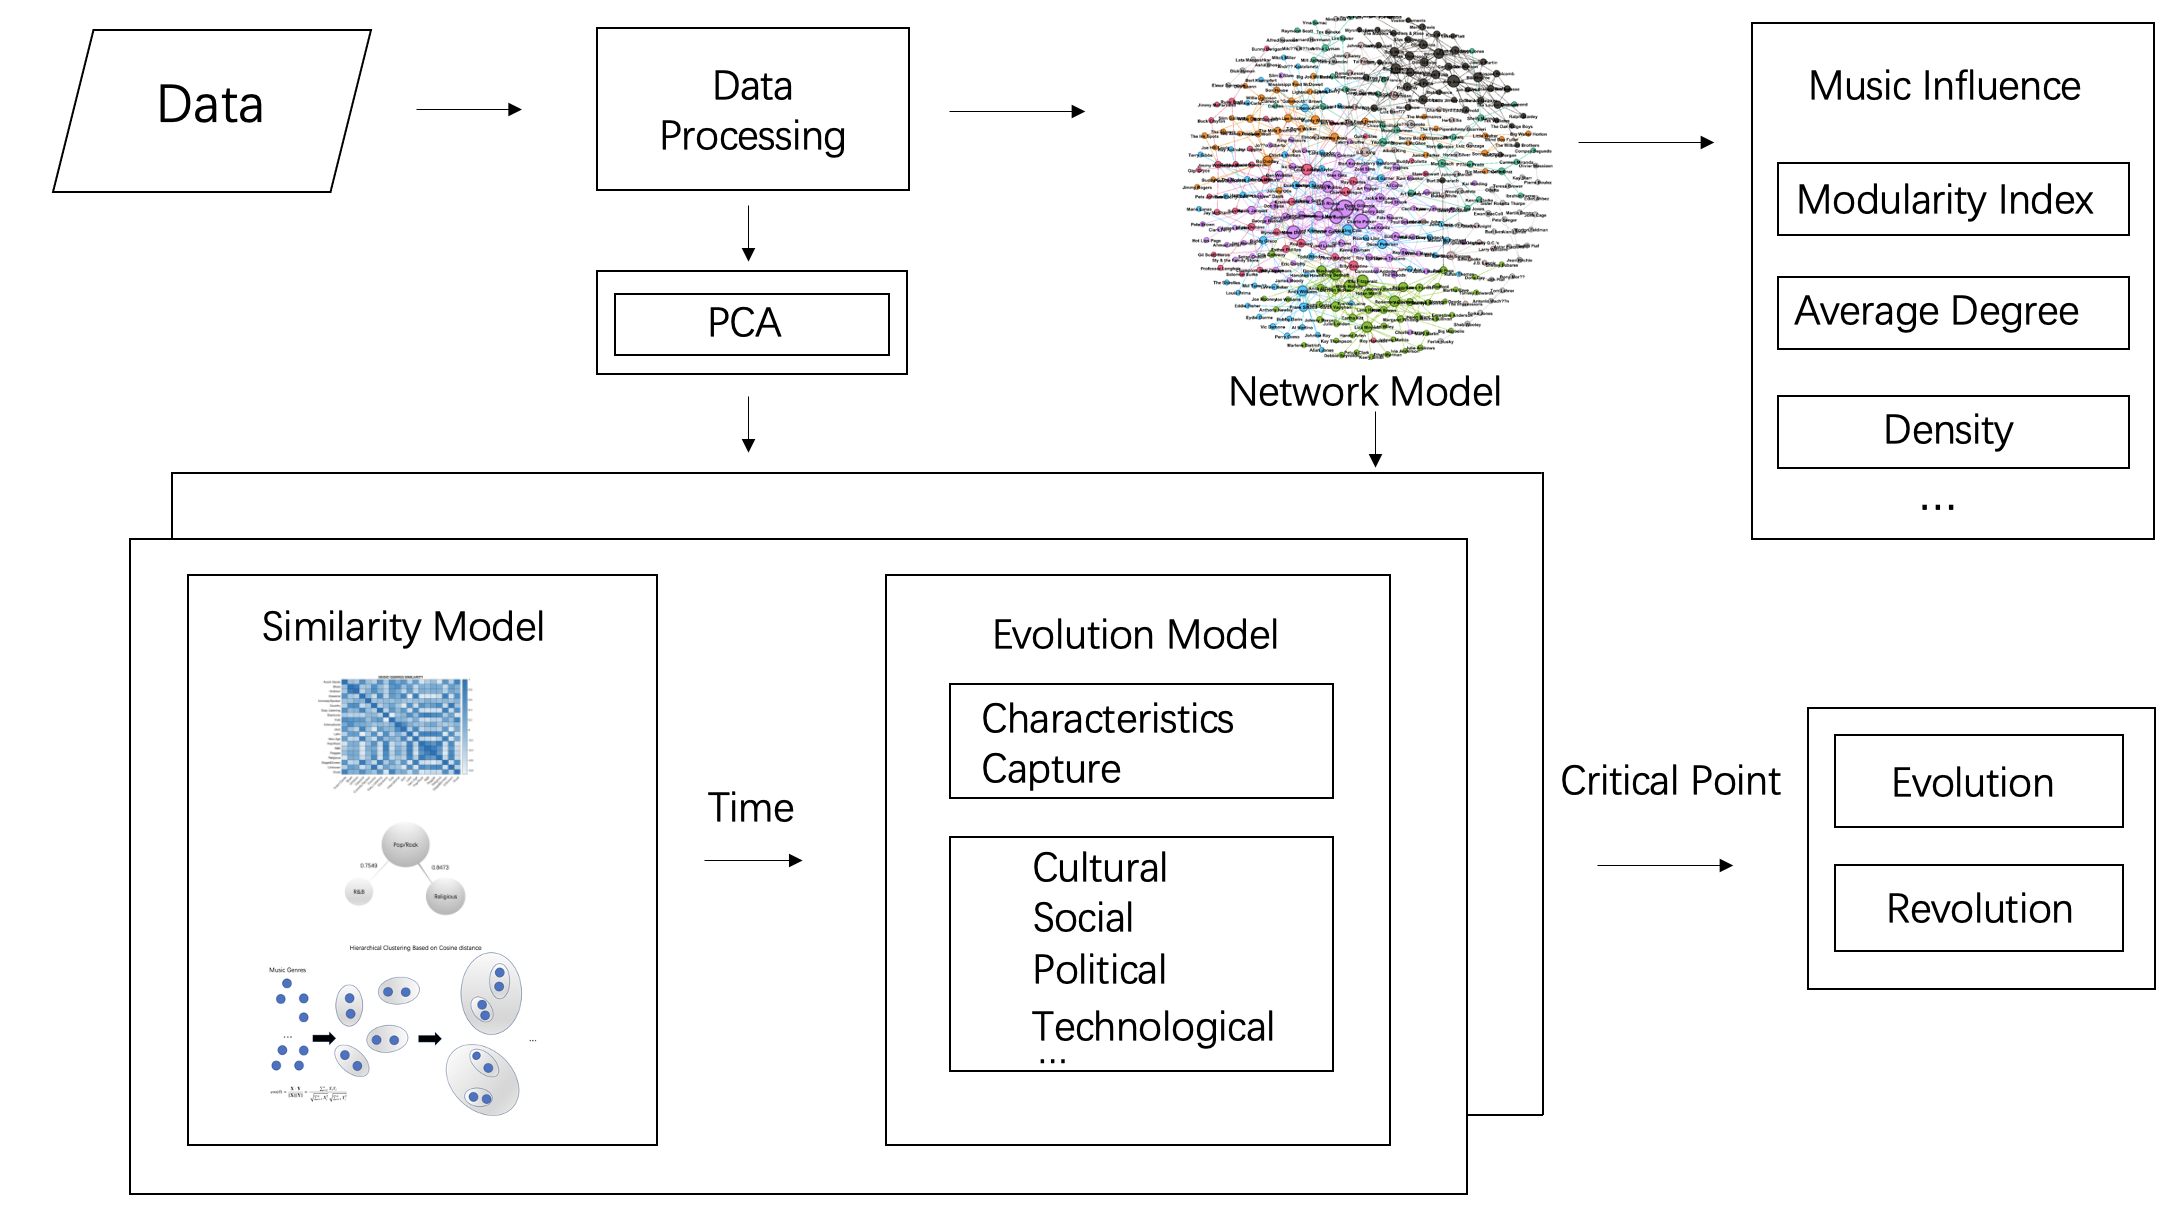
\includegraphics[width=12cm]{Q2_modeloverview.png}
\caption{Main Framework of the Model}
\label{overview}
\end{figure}



\section{Assumptions and Notations}

\subsection{Assumptions}
In our model, we make the following assumptions.
\begin{itemize}
    \item The music genre of artists would not change suddenly.
    \item The main factor with respect to the change of music genre for artists would be the influence of other artists.
    \item There is no overlap of the genre for a certain song, that is, the classification and features of songs are clear.
    \item The basic time unit in our model is considered as one year.
    \item The average level of songs from a certain genre could represent the whole features of the genre.
\end{itemize}

\subsection{Notations}
\begin{minipage}{\textwidth}
\begin{minipage}[t]{0.48\textwidth}
\makeatletter\def\@captype{table}
\begin{tabular}{p{80pt}p{80pt}p{80pt}}
    \toprule
    Notations     & Interpretation\\
    \midrule
    $x_1$     & Danceability\\
	$x_2$  &  Energy\\
	$x_3$  &  Valence\\
	$x_4$  &  Tempo\\
	$x_5$  &  loudness\\
	$x_6$  &  Mode\\
	$x_7$  &  key\\
	$x_8$  &  Acousticness\\
	$x_9$  &  Instrumentalness\\
    \bottomrule
\end{tabular}
\caption{Notations list 1}
\label{Notations list 1}
\end{minipage}
\begin{minipage}[t]{0.48\textwidth}
\makeatletter\def\@captype{table}
\begin{tabular}{p{80pt}p{80pt}p{80pt}}
    \toprule
    Notations     & Interpretation\\
    \midrule
    $x_{10}$  & Liveness\\
	$x_{11}$ &  Speechiness\\
	$x_{12}$ &  Explicit\\
	$x_{13}$  & Durations(ms)\\
	$x_{14}$  &  Popularity\\
	$e_{ii}$  & Ratio of edges\\
	$a_i^2$ & Ratio of edges\\
	$cut(C_i,\ \bar{C_i})$ & Edges\\
	$vol(C_i)$ & Edges\\
    \bottomrule
\end{tabular}
\caption{Notations list 2}
\label{Notations list 2}
\end{minipage}
\end{minipage}


\section{Data Processing}
The data sets given by ICM provide us lots of information for analysis. The attached file \emph{"influence\_data"} contains influencers and followers for 5,854 artists in the last 90 years. The attached file \emph{"full\_music\_data”} provides 16 variable entries, including musical features such as danceability, tempo, loudness, and key, along with other related information for each of 98,340 songs. However, This is a huge amount of data with lots of redundant and useless data, which could be the main obstacle for later analysis. Namely, data processing by cleaning, selecting and standardizing is needed.


\subsection{Data Cleaning}
In order to improve the quality of data, we should detecting and removing errors and inconsistencies from data especially when multiple data sources need to be integrated \cite{article8}. Hence, the following approaches are addressed to solve the problems.
\begin{itemize}
\item Perhaps due to some statistical negligence, places with missing data appear from time to time. Therefore, for variables with a large amount of data missing, we just delete it, which could be explained by the fact that small data cannot provide enough and valuable information for our modeling and analysis. For variables with a small amount of data missing, we use the interpolation method to fill the missing values. \textbf{For instance, some data of the genre of music are missed in the file, which causes the problem that the classification of certain songs fails}. Since this data type is not value but text, the small samples of songs are deleted, which is also consistent with our assumptions. This method is widely used for the file \emph{"full\_music\_data”}.
\item Abnormal values mean that if a value in a set of data is more than twice the standard deviation of the average, we call it the abnormal value. Statistically, we can use a box-plot to identify the abnormal values. For the abnormal value, we fix it with the average value of its two adjacent observations. This method is used for summarising the information of the artist, influencer and follower, respectively.
\end{itemize} 
\subsection{Data standardization}
This step aims to standardize the range of the continuous initial variables so that each one of them contributes equally to the analysis. In other words, to avoid the situation that those variables with larger ranges will dominate over those with small ranges, we need to standardize the data.
Mathematically, this can be done by subtracting the mean and dividing by the standard deviation for each value of each variable.\\

\begin{equation}
z =\frac{x-\mu}{\sigma}
\end{equation}



\textbf{For instance, the feature "duration" in the \emph{"full\_music\_data"} will dominate the conclusion since it has huge magnitude compared with other features}. Therefore, it is really necessary to make sure that the data varies in the same scale by standardizing the data.
\subsection{Data Synthesis and Classification}
Firstly, applying statistical skills, we find that there are 20 genres in total, which is showed below Table \ref{Music Genres} (alphabetical order).
\begin{table} [H]
\begin{center}
\begin{tabular}{p{80pt}p{80pt}p{80pt}}
\toprule
\midrule
Avant-Grade     & Jazz\\
Blues & Latin\\
Children's & New Age\\
Classical & Pop/Rock\\
Comedy/Spoken & R\&B\\
Country & Reggae\\
Easy Listening & Religious\\
Electronic & Stage\& Screen \\
Folk & Unknown\\
International & Vocal\\
\bottomrule
\end{tabular}
\end{center}
\caption{Music Genres}
\label{Music Genres}
\end{table}
Secondly, group the songs from the same genre, and calculate the average value, we could get a matrix containing the basic information of the genres and corresponding features as showed in Figure \ref{Data}.\\
\begin{figure}[H]
\label{fig:aa}
\small
\centering
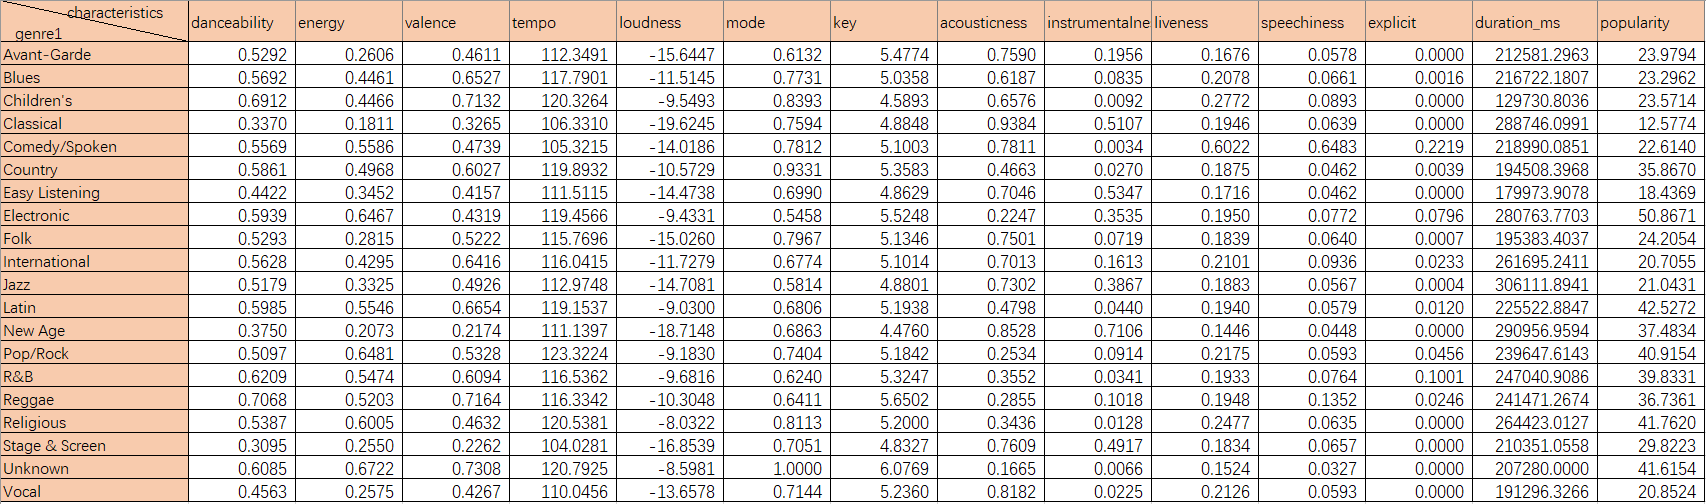
\includegraphics[width=12cm]{figures/Q2_originaldata.png}
\caption{Data classification of the genres and features (Average Level)}
\label{Data}
\end{figure}
Thirdly, standardizing the data by using the formula in 3.2, we could get the below Figure \ref{StData}.
\begin{figure}[H]
\label{fig:aa}
\small
\centering
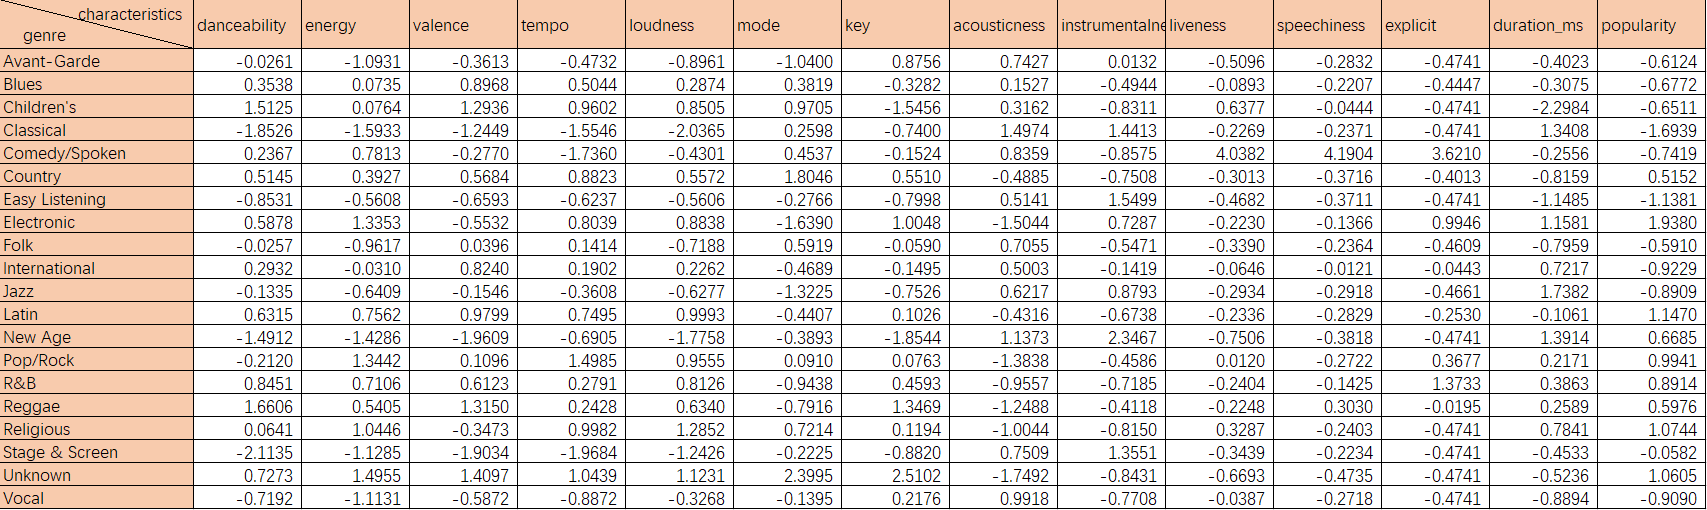
\includegraphics[width=12cm]{figures/Q2_standardizedata.png}
\caption{Standardized Data}
\label{StData}
\end{figure}
The above steps are significant for later analysis, the process of model development could be divided into three categories, which is Network Construction, the Similarity Model of music and Evolution. 
\section{Network Construction}
\subsection{Evaluation Index}
\label{Evaluation Index}
We use Modularity\cite{article3} and Conductance\cite{article4} unsupervised evaluation indicators to evaluate the merits and demerit of communities in network.

\begin{itemize}
\item Modularity

Modularity is used to evaluate the ratio between communities' edges to network's total edges. Defined as below:

\begin{equation}\label{4_Modularity_1}
Q=\ \sum_{i=1}^{k}\left(e_{ii}-a_i^2\right)
\end{equation}

$e_{ii}$ refers to the ratio of $i^{th}$ community's inner edges to network's total edges and $a_i^2$ refers to the ratio of the number of linked edges between community i and other communities to the network's total edges. According to (\ref{4_Modularity_1}), $Q =  [-0.5, 1]$. The larger the Q, the more obvious communities can be found in the network.

\item Conductance

Conductance is used to evaluate the ratio between number of linked edges between communities to community's inner edges. Defined as below:
\begin{equation}\label{4_Conductance_1}
Conductance(C_i)\ =\ \frac{cut(C_i,\ \bar{C_i})}{min{vol(C_i),vol(\bar{C_i})}}
\end{equation}
$cut(C_i,\ \bar{C_i})$ refers to the edges between communities and $vol(C_i)$ refers to the edges in a community. According to (\ref{4_Conductance_1}), $Conductance(C_i)$ = (0,1]. The smaller the $Conductance(C_i)$, the more connected in the community, the less connected between communities, the better the result of community division.

\end{itemize}

\subsection{Diagram and network model}
\label{Diagram and network model}
By applying diagram and network model, we get the number of influencers and followers of all artists as well as the genre of that artist. The top 6 most influential artists are shown in Table \ref{Top 6 Most Influential Artists}: (e.g. \emph{The Beatles} has 615 followers and influenced by other 31 artists, is the most influential artist).
\begin{table} [H] 
\begin{center}
\begin{tabular}{p{80pt}p{120pt}p{60pt}p{60pt}p{80pt}p{80pt}}
\toprule
Artist Name  & Follower & Influencer & Genre & Year\\
\midrule
The Beatles & 615 & 31 & Pop/Rock & 1960\\
Bob Dylan	& 389	& 29 & Pop/Rock& 1960\\
The Rolling Stones & 319 & 39 & Pop/Rock& 1960\\
David Bowie	& 238 &	25 & Pop/Rock& 1960\\
Led Zeppelin &	221 &	24 & Pop/Rock& 1960\\
Jimi Hendrix &	201 & 32 & Pop/Rock& 1960\\
... & ... & ... & ...& ...\\
\bottomrule
\end{tabular}
\end{center}
\caption{Top 6 Most Influential Artists}
\label{Top 6 Most Influential Artists}
\end{table}

Table \ref{Top 6 Most Influential Artists} shows that the top 6 most influential artists are All of them are Pop/Rock artists in 1960.

Apart from that, we can also get the top 1 most influential artist for each year and each genre separately:
\begin{table} [H] 
\begin{center}
\begin{tabular}{p{80pt}p{80pt}p{80pt}p{80pt}}
\toprule
Year & Artist Name & Follower & Genre\\
\midrule
1930 & Hank Williams & 184 & Country\\
1940 & Miles Davis & 160 & Jazz\\
1950 & Marvin Gaye & 169 & R\&B\\
1960 & The Beatles & 615 & Pop/Rock\\
1970 & Sex Pistols & 153 & Pop/Rock\\
1980 & Metallica &	112 & Pop/Rock\\
1990 & Radiohead &	55 & Pop/Rock\\
2000 & Avril Lavigne &	14 & Pop/Rock\\
2010 & Frank Ocean &	3 & R\&B\\
\bottomrule
\end{tabular}
\end{center}
\caption{Top 1 Most Influential Artist Each Year}
\label{Top 1 Most Influential Artist Each Year}
\end{table}

Analysis from Table \ref{Top 1 Most Influential Artist Each Year}, the artists in the Pop/Rock genre are consistently most influential from 1960 to 2000. Consistent with the trend shown in Table \ref{Top 6 Most Influential Artists}.


\begin{table} [H] 
\begin{center}
\begin{tabular}{p{80pt}p{160pt}p{80pt}p{80pt}}
\toprule
Genre & Artist Name & Follower & Year\\
\midrule
Comedy/Spoken & Spike Jones	& 20	&	1930\\
Country & Hank Williams	& 184	&	1930\\
Folk & Pete Seeger	& 47	&	1930\\
Vocal & Billie Holiday &	106	&	1930\\
Blues & Muddy Waters &	113	& 1940\\
Easy Listening & Henry Mancini	& 19 & 	1940\\
Jazz & Miles Davis	& 160	&	1940\\
Stage \& Screen & Ennio Morricone &	30	&	1950\\
Religious & James Cleveland	& 17	&	1950\\
R\&B & Marvin Gaye &	169	&	1950\\
Latin & Antônio Carlos Jobim &	34	&	1950\\
International & João Gilberto &	27	&	1950\\
Children's & Alvin \& the Chipmunks	& 3	&	1950\\
New Age & Mike Oldfield &	16	&	1960\\
Pop/Rock & The Beatles &	615	&	1960\\
Reggae & Lee "Scratch" Perry &	48	&	1960\\
Avant-Garde & Terry Riley	& 34 & 1960\\
Classical & Steve Reich	& 24	&	1960\\
Electronic & Kraftwerk &	108	&	1970\\
Unknown & The Wonder Stuff	& 1	&	1980\\
\bottomrule
\end{tabular}
\end{center}
\caption{Top 1 Most Influential Artist Each Genre}
\label{Top 1 Most Influential Artist Each Genre}
\end{table}

Analysis from Table \ref{Top 1 Most Influential Artist Each Genre}, the artists with most influence focus on 1930 to 1960. In 1950, there are most kinds of influential genres and in 1960, the number of followers is the largest.

\subsection{Network Diagram}
\begin{itemize}
\item Data Used
\textbf{Edge file:}

In the edge file, there are two main data set: source and target. In each edge file, we use all influencers in a certain year as the source and all followers of the source's artists as the target.

\textbf{Node file:}

In the node file, there is only one used data set: id. In each node file, we use non\_redundant influencers in the corresponding edge file as id.


\item Result

\textbf{Average Degree:} Represent the average of the connecting edges of each node.

\textbf{Density:} Represent the density of the diagram.

\textbf{Modularity:} Measure the degree of modularization of the network diagram. A value greater than 0.44 indicates a certain degree of modularization had reached by the network diagram.


By using the data mentioned before, we can get the following measured parameters and network images:

\begin{table} [H] 
\begin{center}
\begin{tabular}{p{80pt}p{80pt}p{80pt}p{80pt}p{80pt}}
\toprule
Year & Average Degree & Density & Modularity\\
\midrule
1930 & 1.8470 & 0.0010 & 0.7030\\
1940 & 2.0410 & 0.0010 & 0.6950\\
1950 & 2.6350 & 0.0010 & 0.6180\\
1960 & 3.811 & 0.0010 & 0.5260\\
1970 & 2.9880 &	0.0010 & 0.6060\\
1980 & 2.7810 &	0.0010 & 0.6570\\
1990 & 2.3060 &	0.0010 & 0.7180\\
2000 & 0.9240 &	0.0020 & 0.8990\\
2010 & 0.6060 &	0.0190 & 0.9000\\
\bottomrule
\end{tabular}
\end{center}
\caption{Directed Networks By Year}
\label{Directed Networks By Year}
\end{table}

\begin{figure}[H]
\label{fig:aa}
\centering
\subfigure[1930]{
\begin{minipage}[t]{0.25\linewidth}
\centering
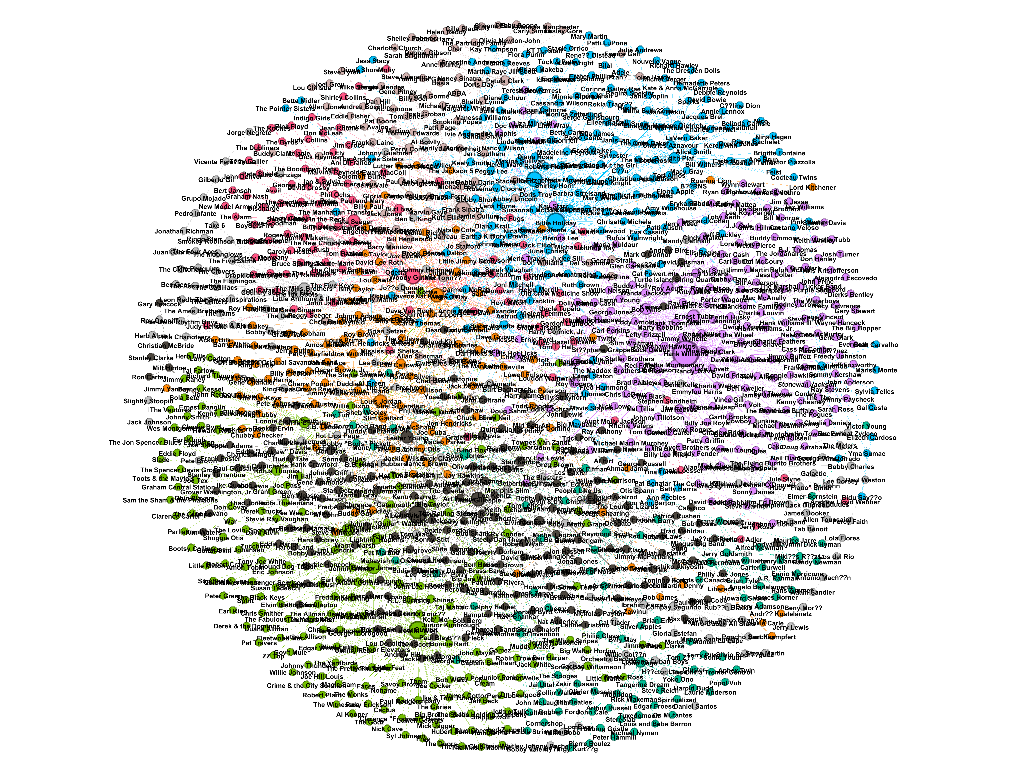
\includegraphics[width=1.7in]{figures/Q1_1930.png}
%\caption{fig1}
\end{minipage}%
}%
\subfigure[1940]{
\begin{minipage}[t]{0.25\linewidth}
\centering
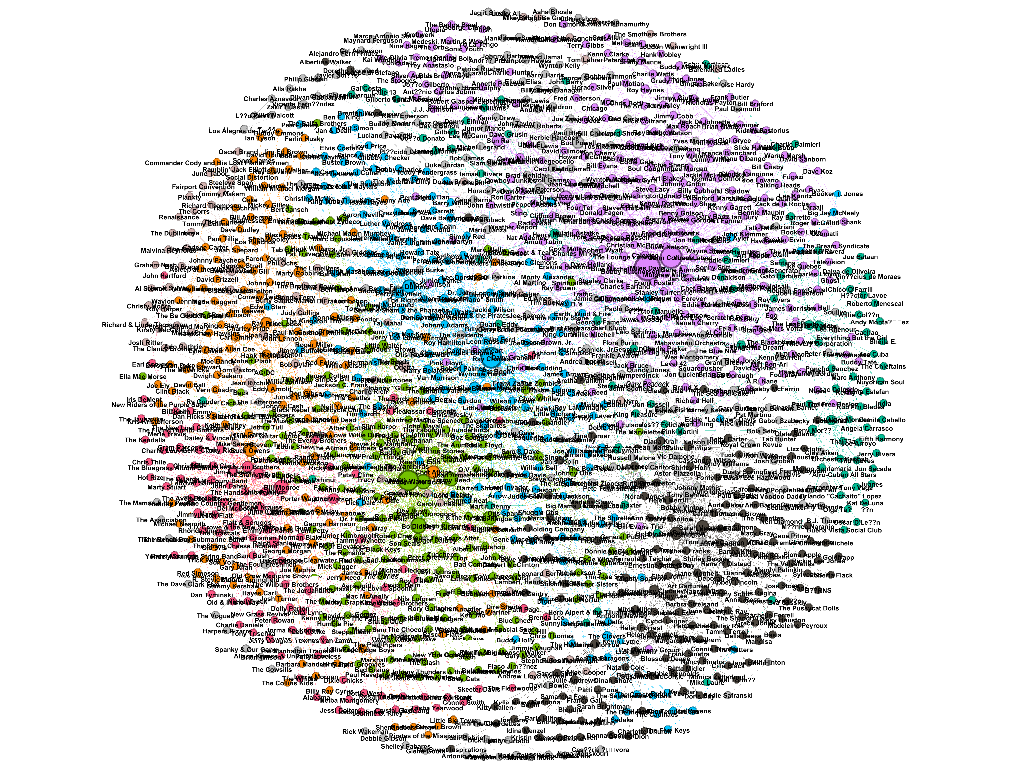
\includegraphics[width=1.7in]{figures/Q1_1940.png}
%\caption{fig2}
\end{minipage}%
}%
\subfigure[1950]{
\begin{minipage}[t]{0.25\linewidth}
\centering
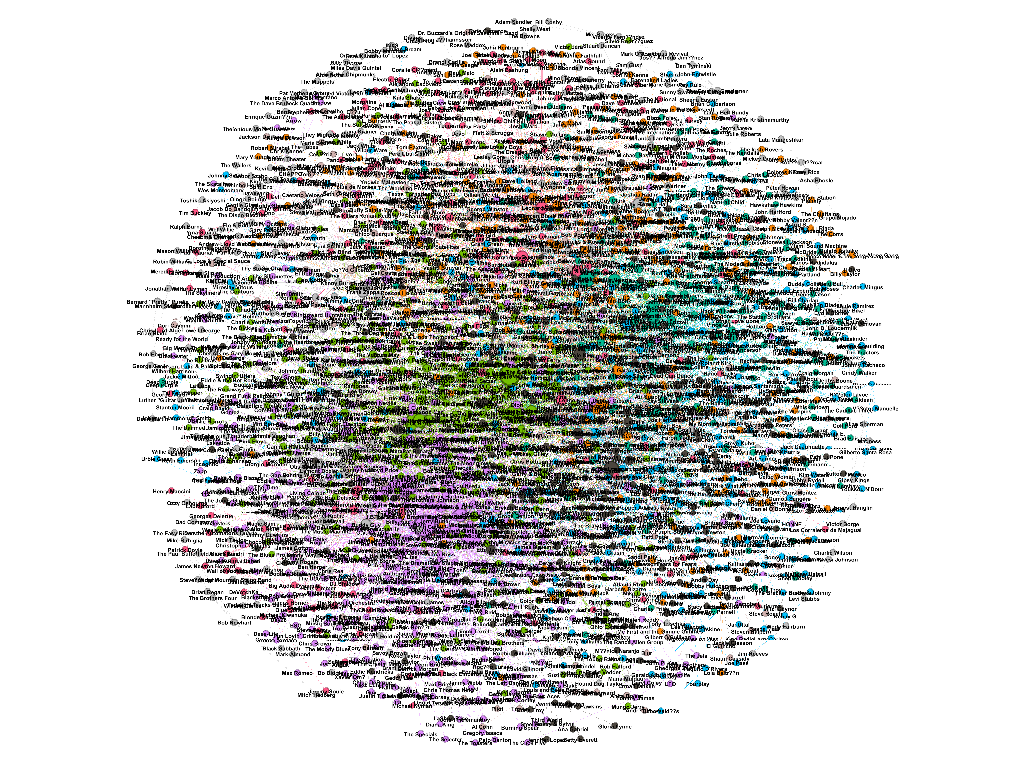
\includegraphics[width=1.7in]{figures/Q1_1950.png}
%\caption{fig2}
\end{minipage}%
}%
\quad
\subfigure[1960]{
\begin{minipage}[t]{0.25\linewidth}
\centering
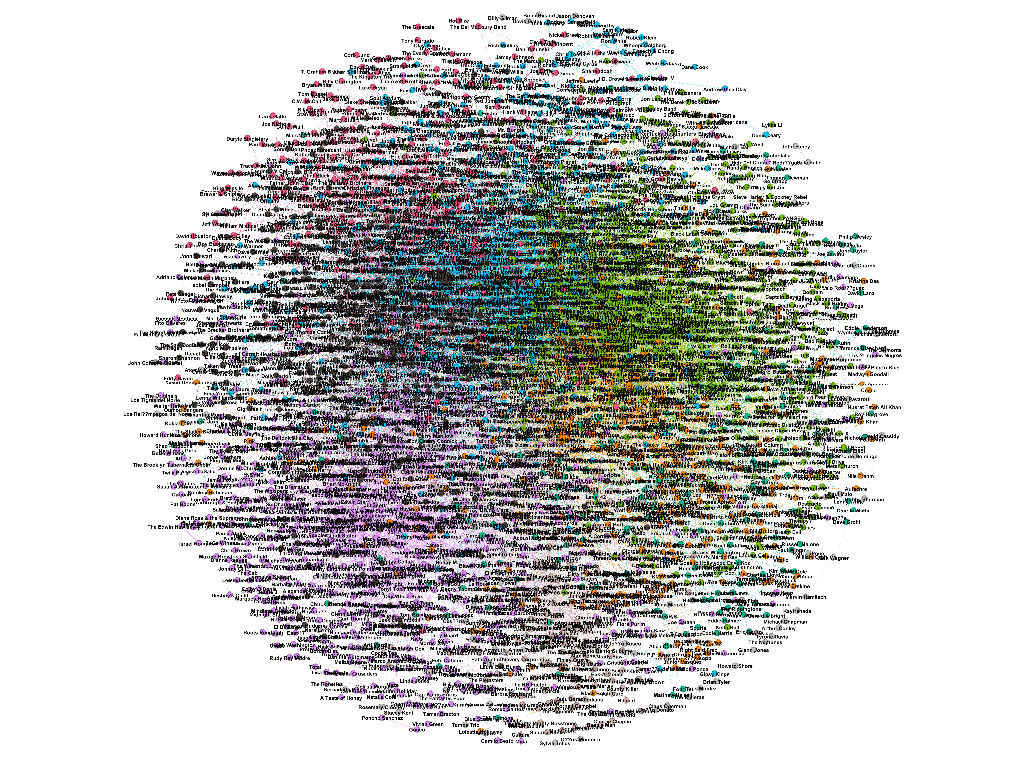
\includegraphics[width=1.7in]{figures/Q1_1960.png}
%\caption{fig2}
\end{minipage}
}%
\subfigure[1970]{
\begin{minipage}[t]{0.25\linewidth}
\centering
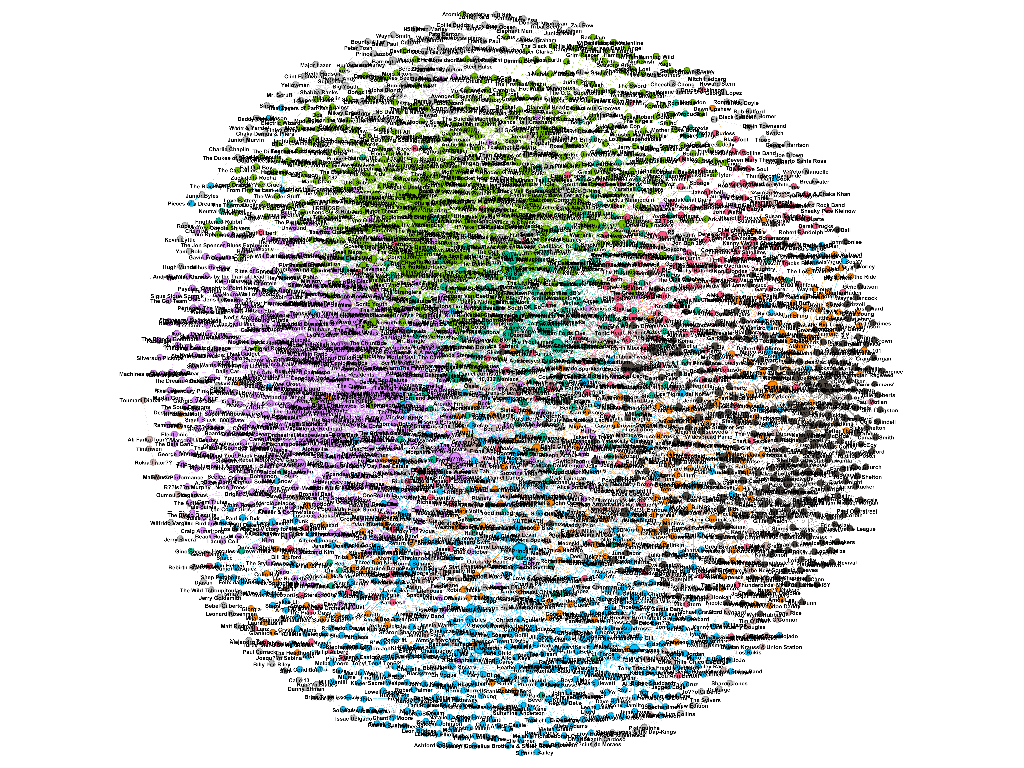
\includegraphics[width=1.7in]{figures/Q1_1970.png}
%\caption{fig2}
\end{minipage}
}%
\subfigure[1980]{
\begin{minipage}[t]{0.25\linewidth}
\centering
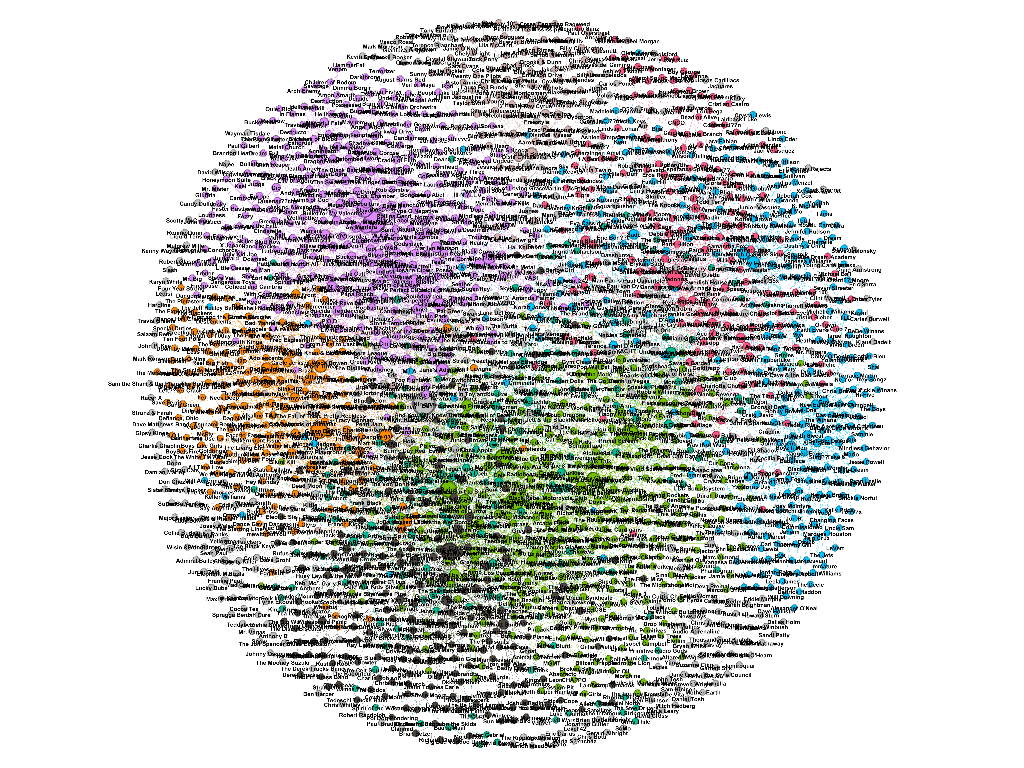
\includegraphics[width=1.7in]{figures/Q1_1980.png}
%\caption{fig2}
\end{minipage}%
}%
\quad
\subfigure[1990]{
\begin{minipage}[t]{0.25\linewidth}
\centering
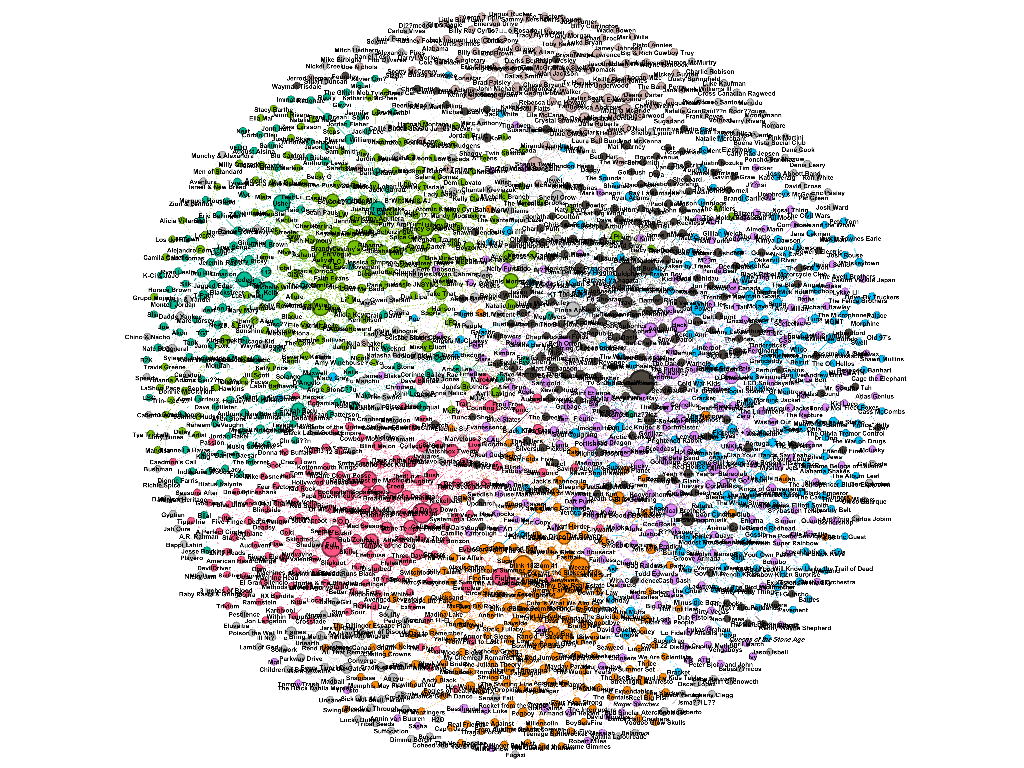
\includegraphics[width=1.7in]{figures/Q1_1990.png}
%\caption{fig2}
\end{minipage}
}%
\subfigure[2000]{
\begin{minipage}[t]{0.25\linewidth}
\centering
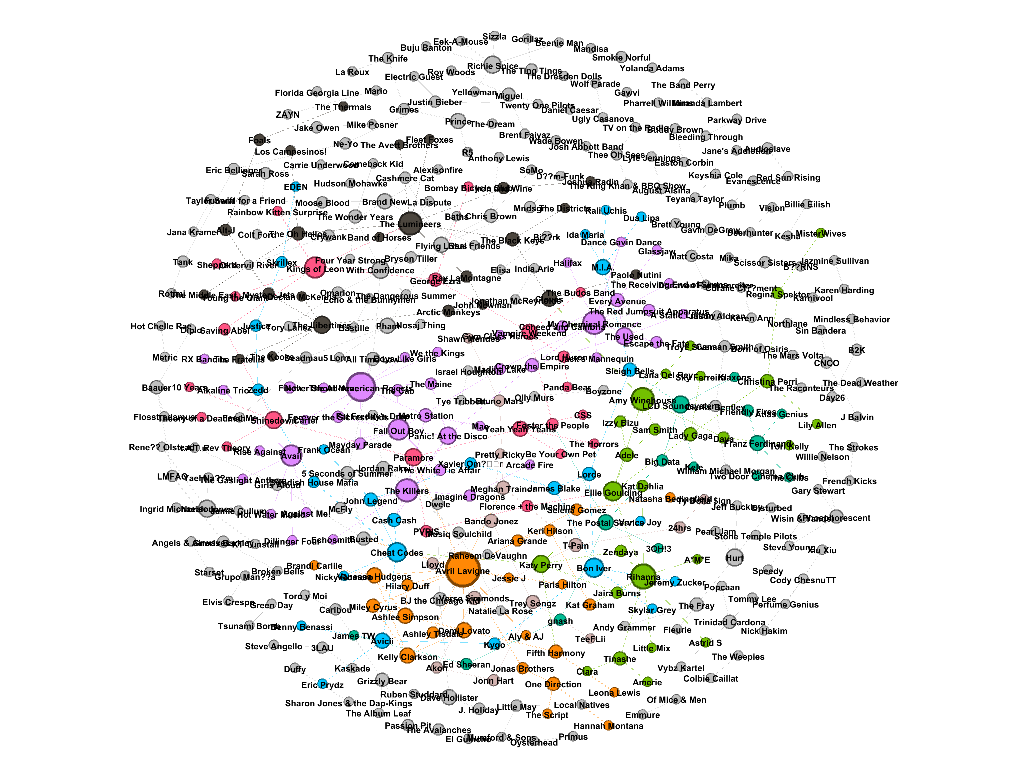
\includegraphics[width=1.7in]{figures/Q1_2000.png}
%\caption{fig2}
\end{minipage}
}%
\subfigure[2010]{
\begin{minipage}[t]{0.25\linewidth}
\centering
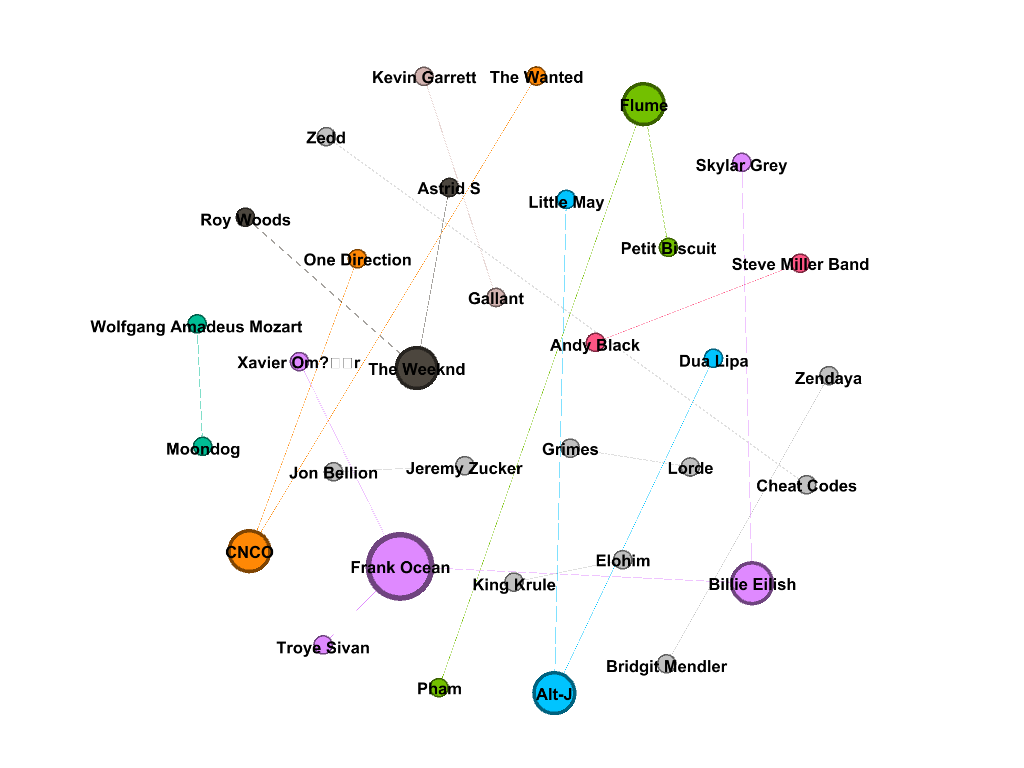
\includegraphics[width=1.7in]{figures/Q1_2010.png}
%\caption{fig2}
\end{minipage}%
}%
\centering
\caption{Network Images By Year}
\label{Network Images By Year}
\end{figure}

\end{itemize}


\textbf{number of edges:} Represent "music influence".

\textbf{nodes:} Represent artists.

Figure \ref{Network Images By Year} shows "music influence" among all artists in each 10 year from 1930 to 2010, nodes are artists and edges between nods are “music influence”. We could find the artist has most complicated edges (music influence) for other years, all detailed images are shown in Figure \ref{Detail Network Images}. 


Taking year 1960 as an example, \emph{"The Beatles"} is the most influential artist. As shown in Figure \ref{Detail Network Images} (d), the biggest blue circle represents \emph{“The Beatles”}. It has the most complicated edges (music influence) and influences a large number of other nodes (artists), which means \emph{"The Beatles"} has the most mutual influencers (influencers + followers).


\begin{figure}[H]
\label{fig:aa}
\centering
\subfigure[1930 - Hank Williams]{
\begin{minipage}[t]{0.25\linewidth}
\centering
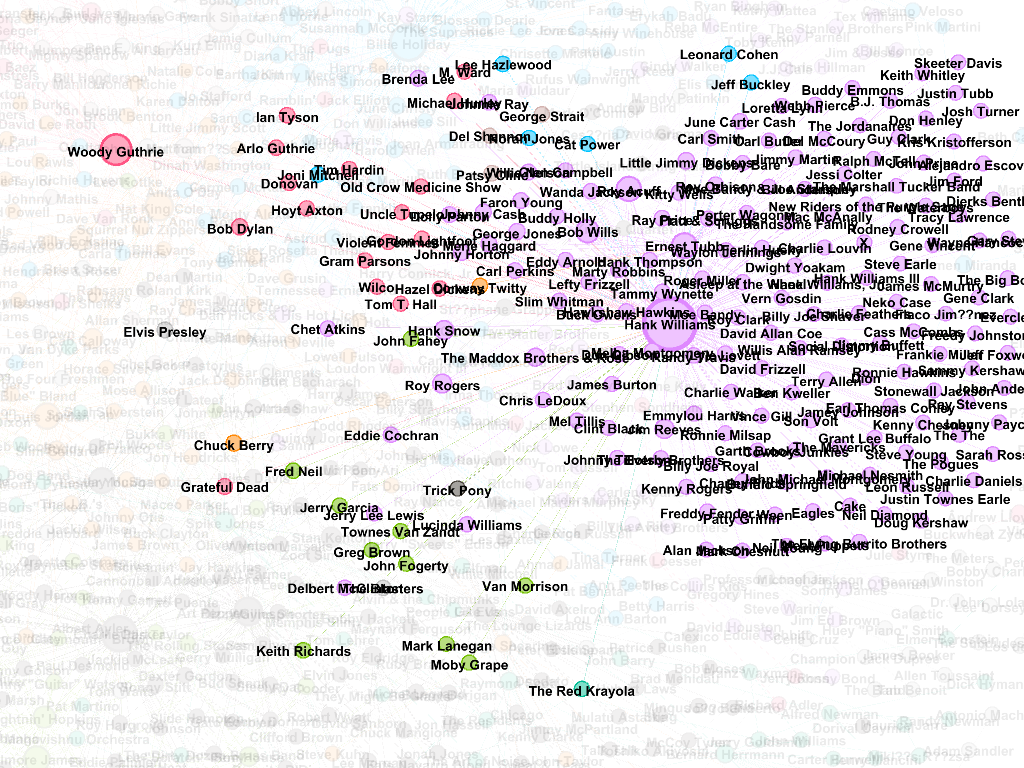
\includegraphics[width=1.7in]{figures/Q1_1930_Artist.png}
%\caption{fig1}
\end{minipage}%
}%
\subfigure[1940 - Miles Davis]{
\begin{minipage}[t]{0.25\linewidth}
\centering
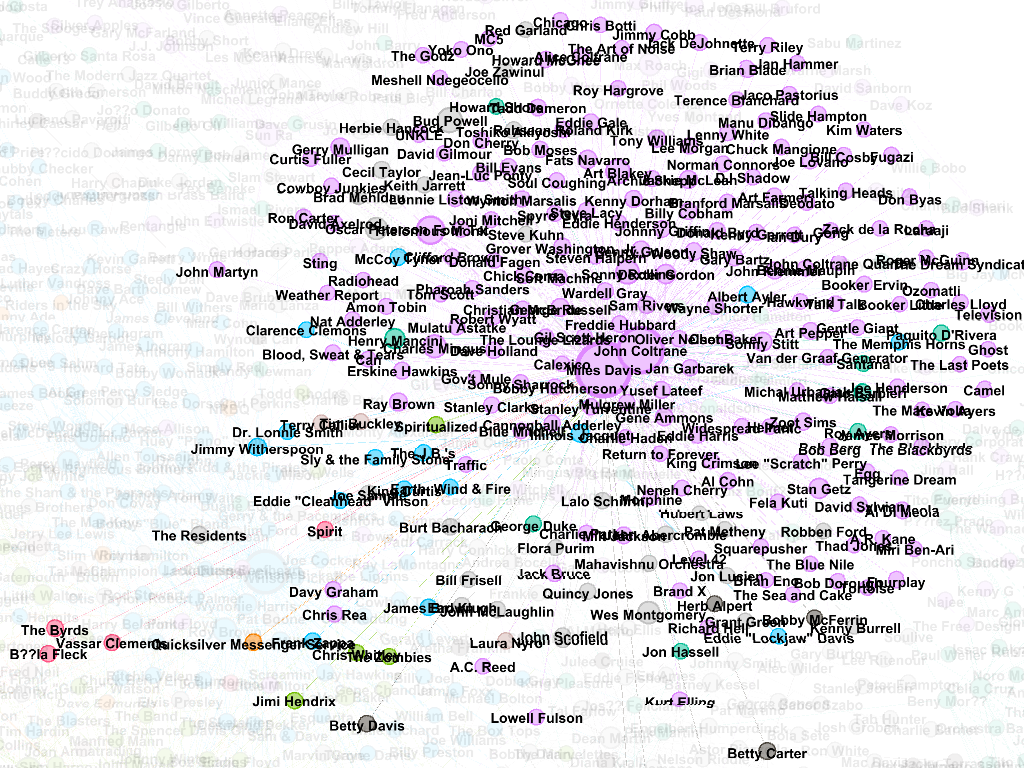
\includegraphics[width=1.7in]{figures/Q1_1940_Artist.png}
%\caption{fig2}
\end{minipage}%
}%
\subfigure[1950 - Marvin Gaye]{
\begin{minipage}[t]{0.25\linewidth}
\centering
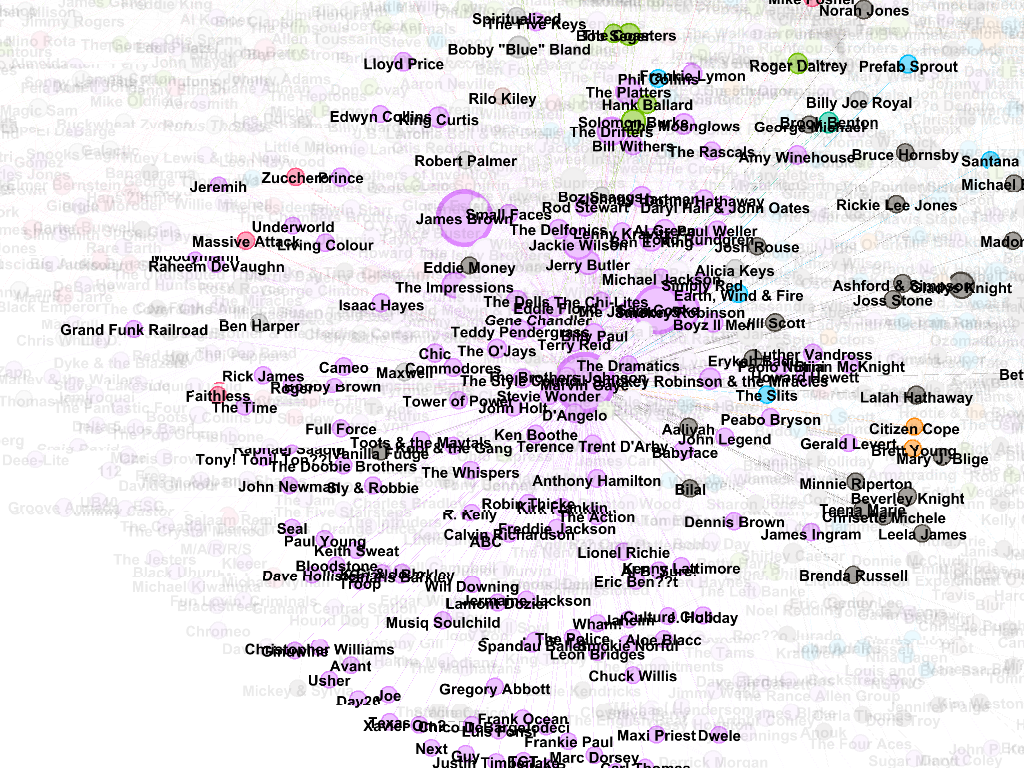
\includegraphics[width=1.7in]{figures/Q1_1950_Artist.png}
%\caption{fig2}
\end{minipage}%
}%
\quad
\subfigure[1960 - The Beatles]{
\begin{minipage}[t]{0.25\linewidth}
\centering
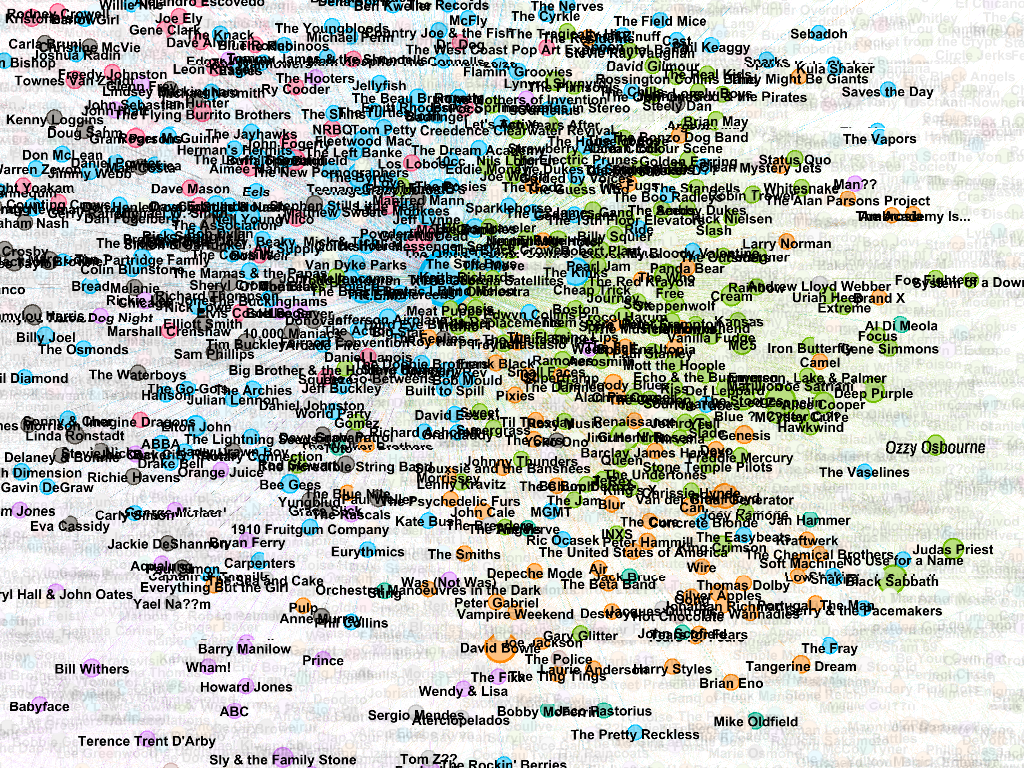
\includegraphics[width=1.7in]{figures/Q1_1960_Artist.png}
%\caption{fig2}
\end{minipage}
}%
\subfigure[1970 - Sex Pistols]{
\begin{minipage}[t]{0.25\linewidth}
\centering
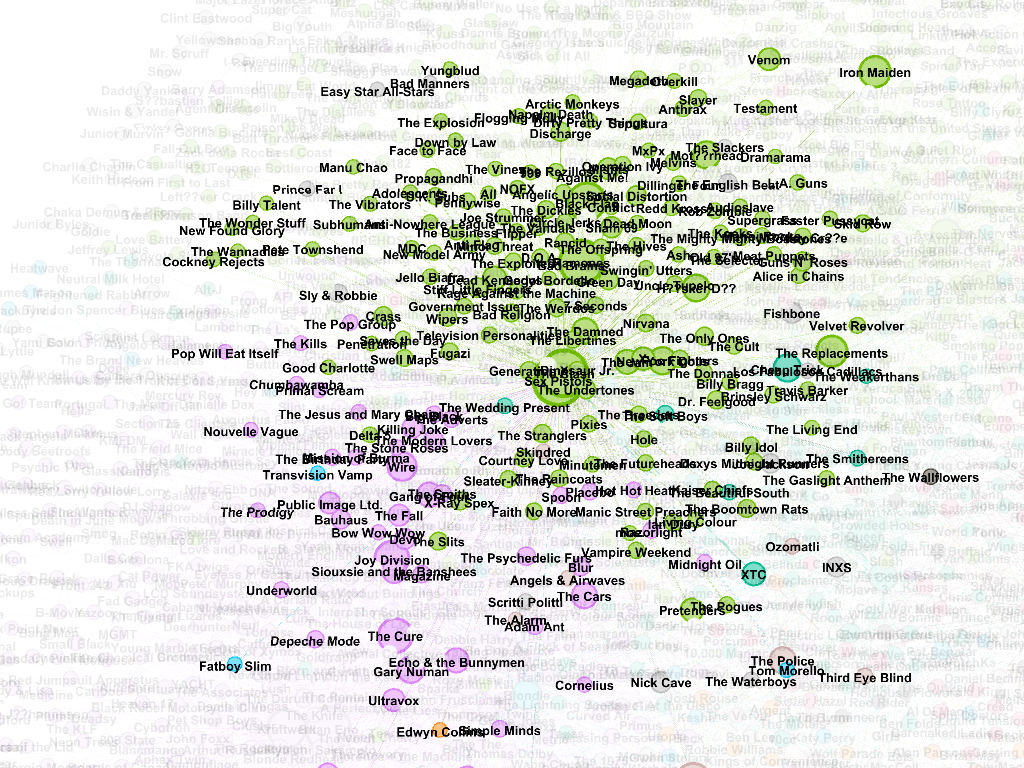
\includegraphics[width=1.7in]{figures/Q1_1970_Artist.png}
%\caption{fig2}
\end{minipage}
}%
\subfigure[1980 - Metallica]{
\begin{minipage}[t]{0.25\linewidth}
\centering
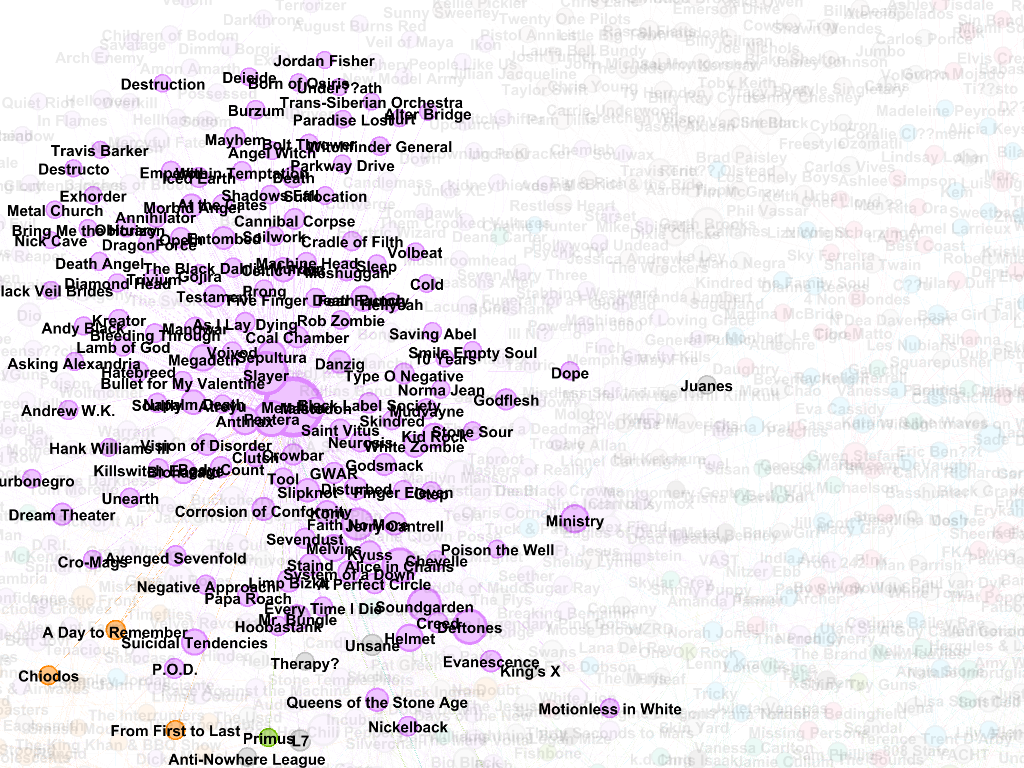
\includegraphics[width=1.7in]{figures/Q1_1980_Artist.png}
%\caption{fig2}
\end{minipage}%
}%
\quad
\subfigure[1990 - Radiohead ]{
\begin{minipage}[t]{0.25\linewidth}
\centering
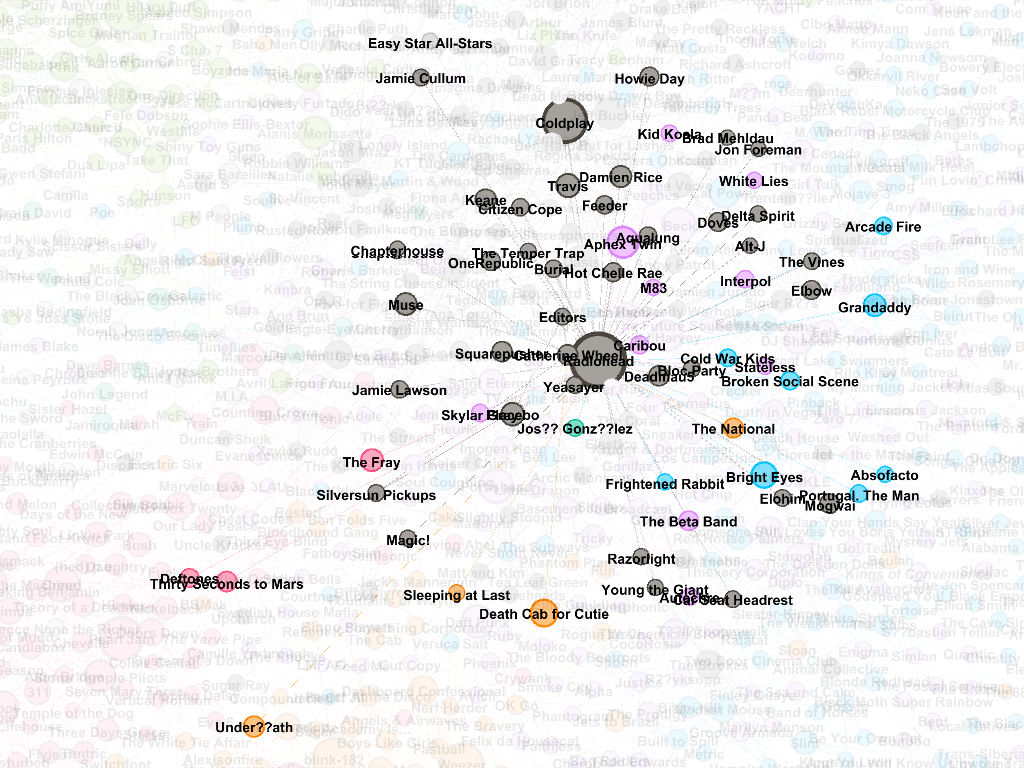
\includegraphics[width=1.7in]{figures/Q1_1990_Artist.png}
%\caption{fig2}
\end{minipage}
}%
\subfigure[2000 - Avril Lavigne]{
\begin{minipage}[t]{0.25\linewidth}
\centering
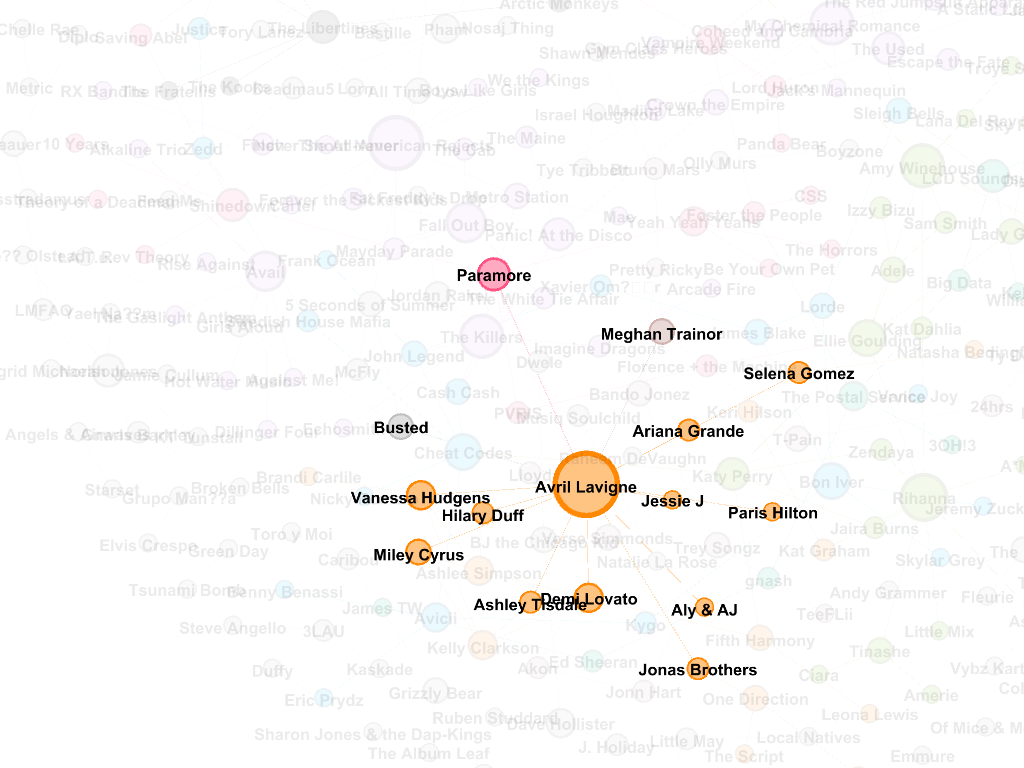
\includegraphics[width=1.7in]{figures/Q1_2000_Artist.png}
%\caption{fig2}
\end{minipage}
}%
\subfigure[2010 - Frank Ocean]{
\begin{minipage}[t]{0.25\linewidth}
\centering
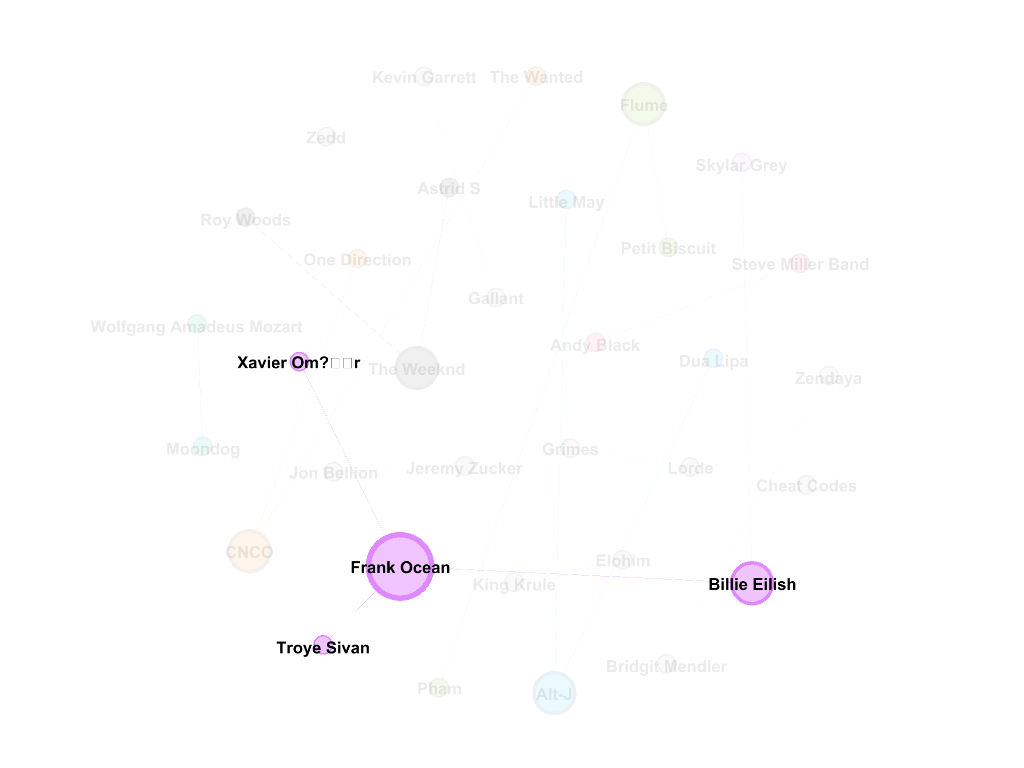
\includegraphics[width=1.7in]{figures/Q1_2010_Artist.png}
%\caption{fig2}
\end{minipage}%
}%
\centering
\caption{Detail Network Images}
\label{Detail Network Images}
\end{figure}

The layout of all images in Figure \ref{Detail Network Images} accord with the result shown in Table \ref{Top 1 Most Influential Artist Each Year}. For instance, in 1960s, \emph{"The Beatles"} dominates the music community and it is easy to remind us of the background of that period. Based on this idea, we really need to continue our study on the characteristics of each music genre so that the conclusion will be more precise. Hence, the next section mainly focuses on the characteristics of genre based on the similarity model.

\section{The Similarity Model of Music}
\subsection{PCA analysis}
Since the data has so many dimensions, we introduce the Principal Components Analysis (PCA) to reduce the dimensions.
\begin{itemize}
    \item Standardize the data\\
    We have 14 feature, $x_1 x_2...x_{14}$, representing the danceability, energy...popularity, respectively, and 20 music genres in total. 
    Once the standardization is done, all the variables will be transformed to the same scale. Let $a_{ij}$ be the entry of the data matrix. Standardize the data from $a_{ij}$ to $\hat{a}_{ij}$\\
    
    \begin{equation}
    \hat{a}_{ij}=\frac{a_{ij}-\mu}{s_j}
    \end{equation}
    where $i=1,2,...20;j=1,2,...,14$
    
    \begin{equation}
    \mu_j=\frac{1}{n}\sum_{i=1}^{n}a_{ij};s_j=\sqrt{\frac{1}{n-1}\sum_{i=1}^{n}(a_{ij}-\mu_j)^2}
    \end{equation}

    
    \item Calculate the correlation coefficient matrix
    $R=(r_{ij})_{14\times14}$, 
    $r_{ij}=\frac{\sum_{k=1}^n a_{ki}a_{kj}}{n-1},i,j=1,2,...14,r_{ii}=1$
    which is visualized as Figure \ref{corrmatrix}.\\
    
    \item Calculate the eigenvalues $\lambda$ and eigenvector $u$. \\
    \item Choose the principal components \\
    By calculating the contribution of each component, we could figure out the contribution rate and cumulative contribution rate.
    
    \begin{equation}
    b_j=\frac{\lambda_j}{\sum_{k=1}^{14}\lambda_k},j=1,2,...,14
    \end{equation}
    
    \begin{equation}
    \alpha_p=\frac{\sum_{k=1}^p\lambda_k}{\sum_{k=1}^{14}\lambda_k}
    \end{equation}

    where $p$ is the number of components we choose, which is shown in Figure \ref{contr}.\\
    
    

\begin{figure}[H]
\centering
\begin{minipage}[t]{0.48\textwidth}
\centering
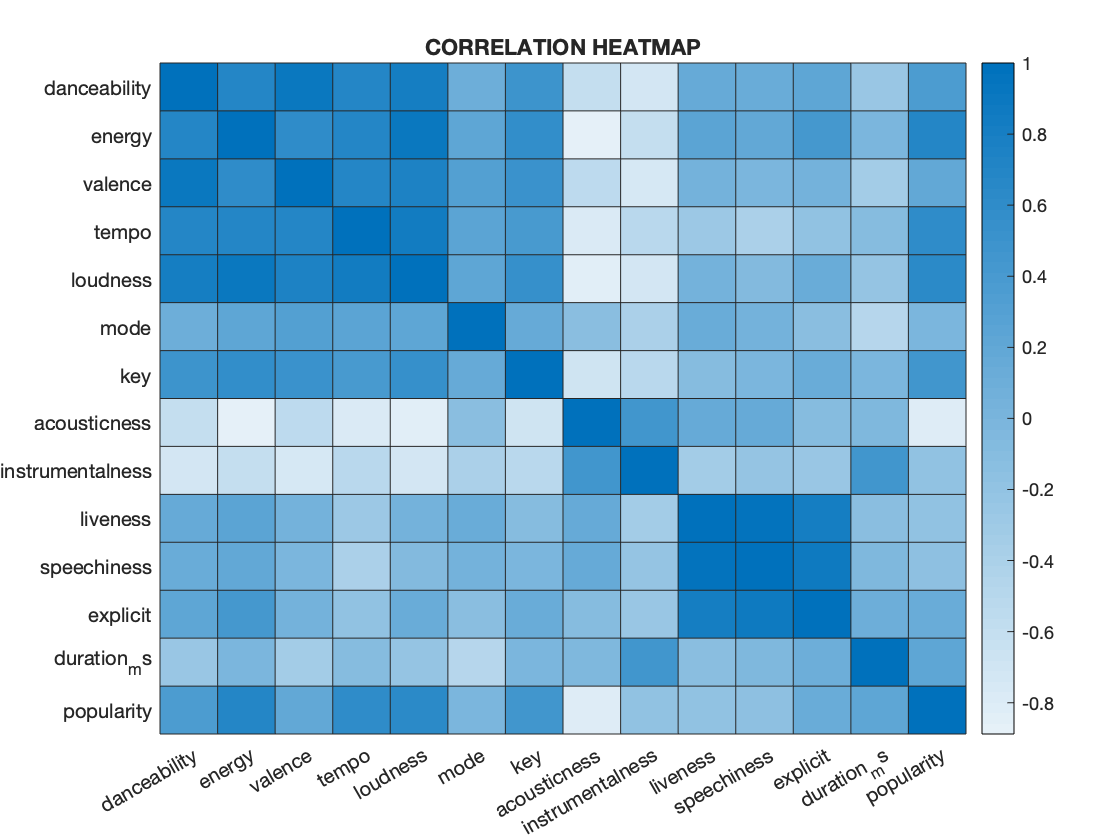
\includegraphics[width=8cm]{Q2_corrheatmap.png}
\label{corrmatrix}
\caption{correlation matrix}
\end{minipage}
\begin{minipage}[t]{0.48\textwidth}
\centering
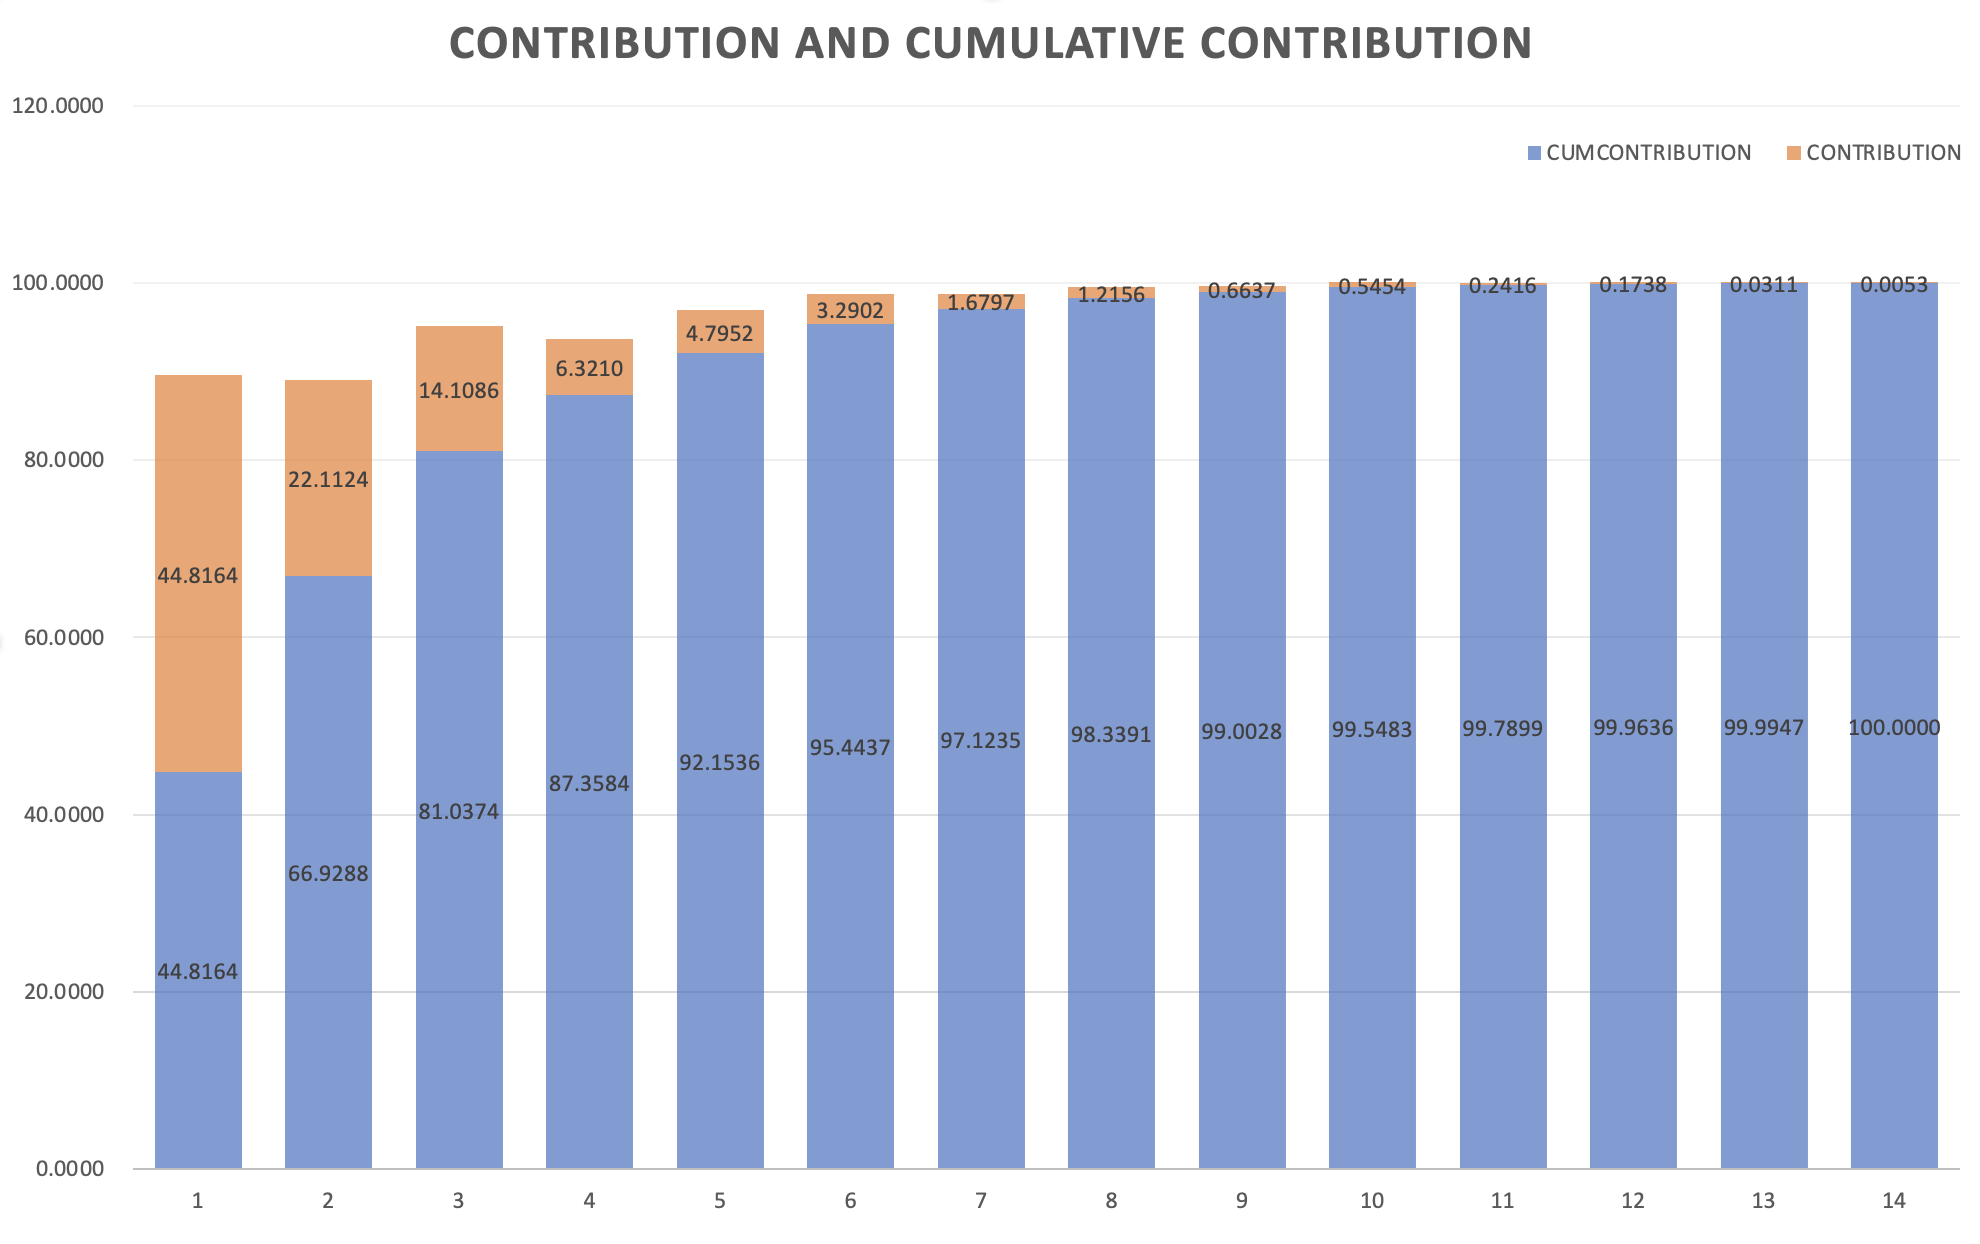
\includegraphics[width=8cm]{figures/Q2_cumcontr.png}
\caption{Contribution rate and Cumulative contribution rate}
\label{contr}
\end{minipage}
\end{figure}

    \item Calculate the scores
    
    \begin{equation}
    Z=\sum_{j=1}^p b_jy_j
    \end{equation}

    
\end{itemize}
\textbf{Result of PCA}:
As the correlation map shows, there exists a very closed relationship between some factors. If we use these factors directly, it will cause the overlap of information, which could also affect the final result. By PCA, we could reduce the dimension of the data and analyze the data more precisely. As the cumulative contribution rate shows, we choose the first 4 components, that is the $\alpha_p=0.85$. \\
\begin{table} [H]
\begin{center}
\begin{tabular}{p{80pt}p{80pt}p{80pt}}
\toprule
\midrule
Eigenvalues     & Contribution Rate & Cumulative Contribution Rate\\
6.2743 & 44.8164 & 44.8164\\
3.0957 & 22.1124 &66.9288\\
1.9752 & 14.1086 &81.0374\\
0.8849 & 6.3210 & 87.3584\\
\bottomrule
\end{tabular}
\end{center}
\caption{The First 4 Components}
\label{The first 4 componets}
\end{table}

\begin{table} [H]
\begin{center}
\begin{tabular}{|c|c|c|c|c|c|c|c|c|c|c|c|c|c|}
\toprule
\midrule
$x_1$&$x_2$&$x_3$&$x_4$ & $...$ & $x_{14}$\\
0.3423&0.0738&-0.0815&-0.4312& $..$& 0.2453 \\
0.3626&0.0910&0.1955&0.1568&$...$&0.6484\\
0.3277&0.0099&-0.2514&-0.3675&$...$&-0.2808 \\
0.3316&-0.2278&-0.0318&-0.0623&$...$&-0.1457 \\
\bottomrule
\end{tabular}
\end{center}
\caption{The Corresponding Eigenvectors (Excerpt)}
\label{Eigenvectors}
\end{table}

By calculating the scores, we could get the score which is showed in table \ref{scores}. 
\begin{equation}
Z=44.8164y_1+22.1124y_2+14.1086y_3+6.3210y_4
\end{equation}

\begin{table} [H]
\begin{center}
\begin{tabular}{cc}
\toprule
\midrule
Unknown&0.9470\\
Comedy/Spoken&0.8314\\
Electronic&0.8229\\
Pop/Rock&0.7999\\
R\&B &0.7927\\
Reggae&0.7881\\
Religious&0.7600\\ 
\bottomrule
\end{tabular}
\end{center}
\caption{The scores}
\label{scores}
\end{table}
With the top scores of PCA, the corresponding genres are unknown, Comedy/Spoken, electronic, Pop/Rock, R\&B, Reggae and Religious, next, we will mainly explore these genres. Once the PCA is done, the complexity of the data has been reduced and we could consider the features which share closed relations so that the similarity model could be more precise. PCA could increase the efficiency of the data given the processes taking place in a smaller dimension \cite{article9}. Then, the next section is about how we use the cosine distance as a measurement for the similarity among music genres after PCA.


\subsection{Measurement of Similarity}
Cosine similarity is a measure of similarity between two non-zero vectors of an inner product space, which could be explained by the following formula:\\


\begin{equation}
\text { Similarity }=\cos (\theta)=\frac{\mathbf{X} \cdot \mathbf{Y}}{\|\mathbf{X}\|\|\mathbf{Y}\|}=\frac{\sum_{i=1}^{n} X_{i} Y_{i}}{\sqrt{\sum_{i=1}^{n} X_{i}^{2}} \sqrt{\sum_{i=1}^{n} Y_{i}^{2}}}
\end{equation}

where $X$ and $Y$ are two non-zero vectors.
Graphically, the cosine similarity measures the direction of two angles in the inner space, which is a judgment of orientation and not magnitude. We introduce this measurement to our model to explore the similarity among music genres.
The relative data is Table \ref{StData}, which is the standardized data. After the calculation, we could visualize the similarity by using the heat map, which is the Figure \ref{music_similarity}.

\begin{figure}[H]
\centering
\begin{minipage}[t]{0.48\textwidth}
\centering
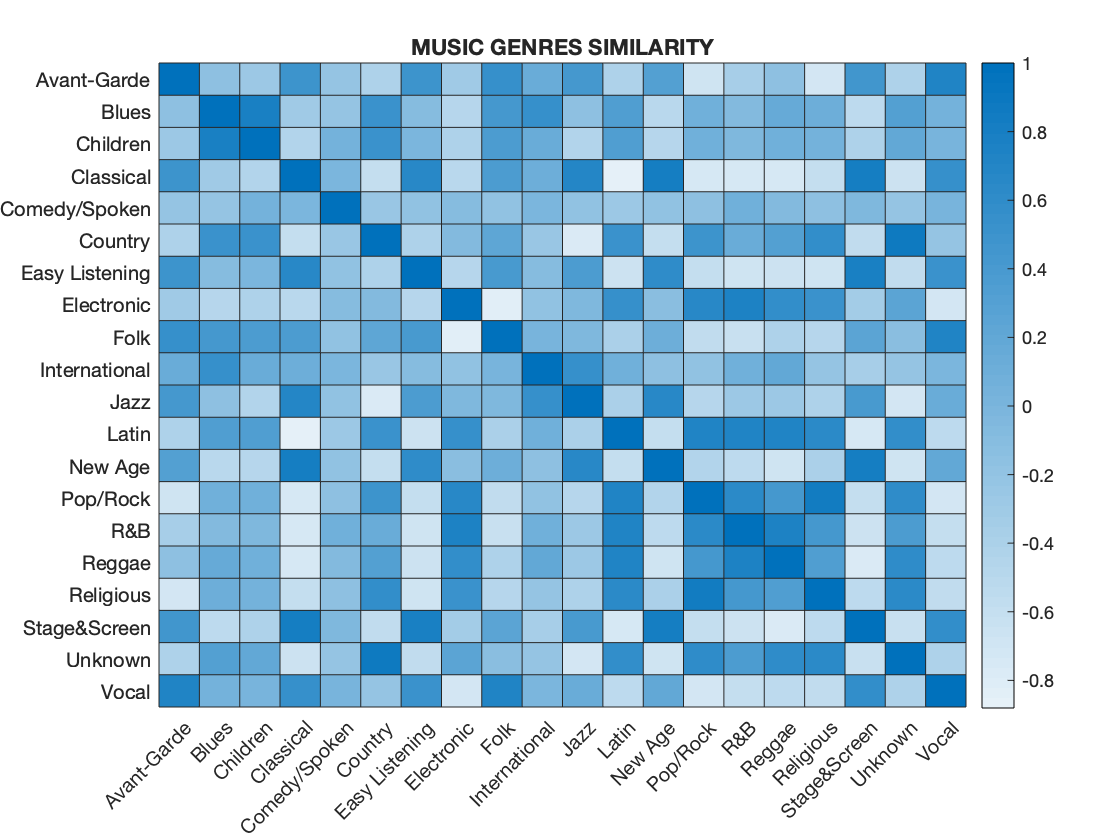
\includegraphics[width=8cm]{Q2_music_similarity.png}
\label{music_similarity}
\caption{Music Genres Similarity}
\end{minipage}
\begin{minipage}[t]{0.48\textwidth}
\centering
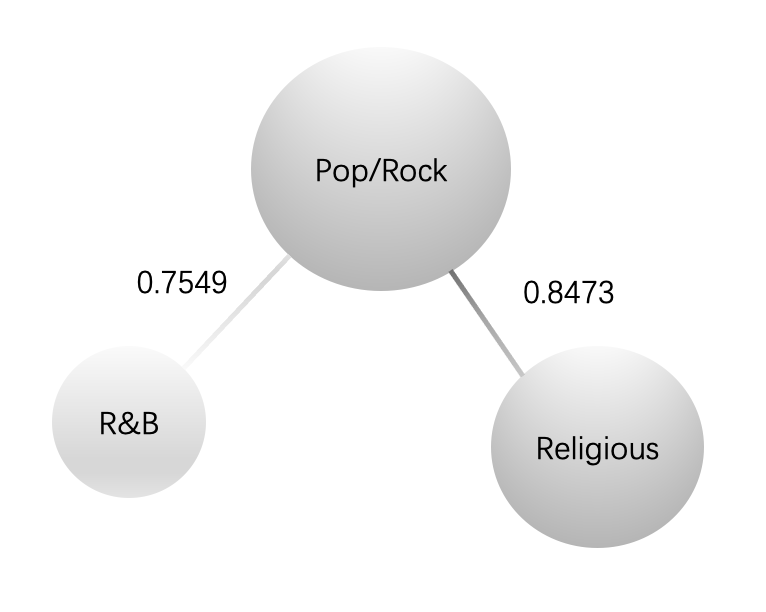
\includegraphics[width=8cm]{figures/Q2_coefficient.png}
\caption{Highest Coefficient}
\label{Highest Coefficient}
\end{minipage}
\end{figure}






It is obvious that Pop/Rock, R\&B, Reggae and Religious are concentrated, which means that those music genres share a very close similarity. Numerically, the similarity between the R\&B and Religious is 0.7549 and the similarity between the Pop/Rock and religious is 0.8473. However, the highest similarity lies between the country and unknown up to 0.8753. Since we could not figure out what genres the unknown music would be, it might be inconclusive for us until we consider the timeline for further study.

The cosine distance gives us a very good measurement for clustering. The next section will present how we use the cosine similarity to clustering the music genres.
\subsection{Hierarchical Clustering}
The hierarchical clustering calculates the similarity between two types of data points, combines the two most similar data points among all data points, and iterates the process repeatedly. To put it simply, hierarchical clustering is to determine the similarity between the data points of each category by calculating the distance between them and all the data points. The smaller the distance, the higher the similarity. The two nearest data points or categories are combined to generate a cluster tree.

The below graph Figure \ref{hclusterrationale} shows the basic rationale of hierarchical clustering based on cosine similarity.



\begin{figure}[H]
\centering
\begin{minipage}[t]{0.48\textwidth}
\centering
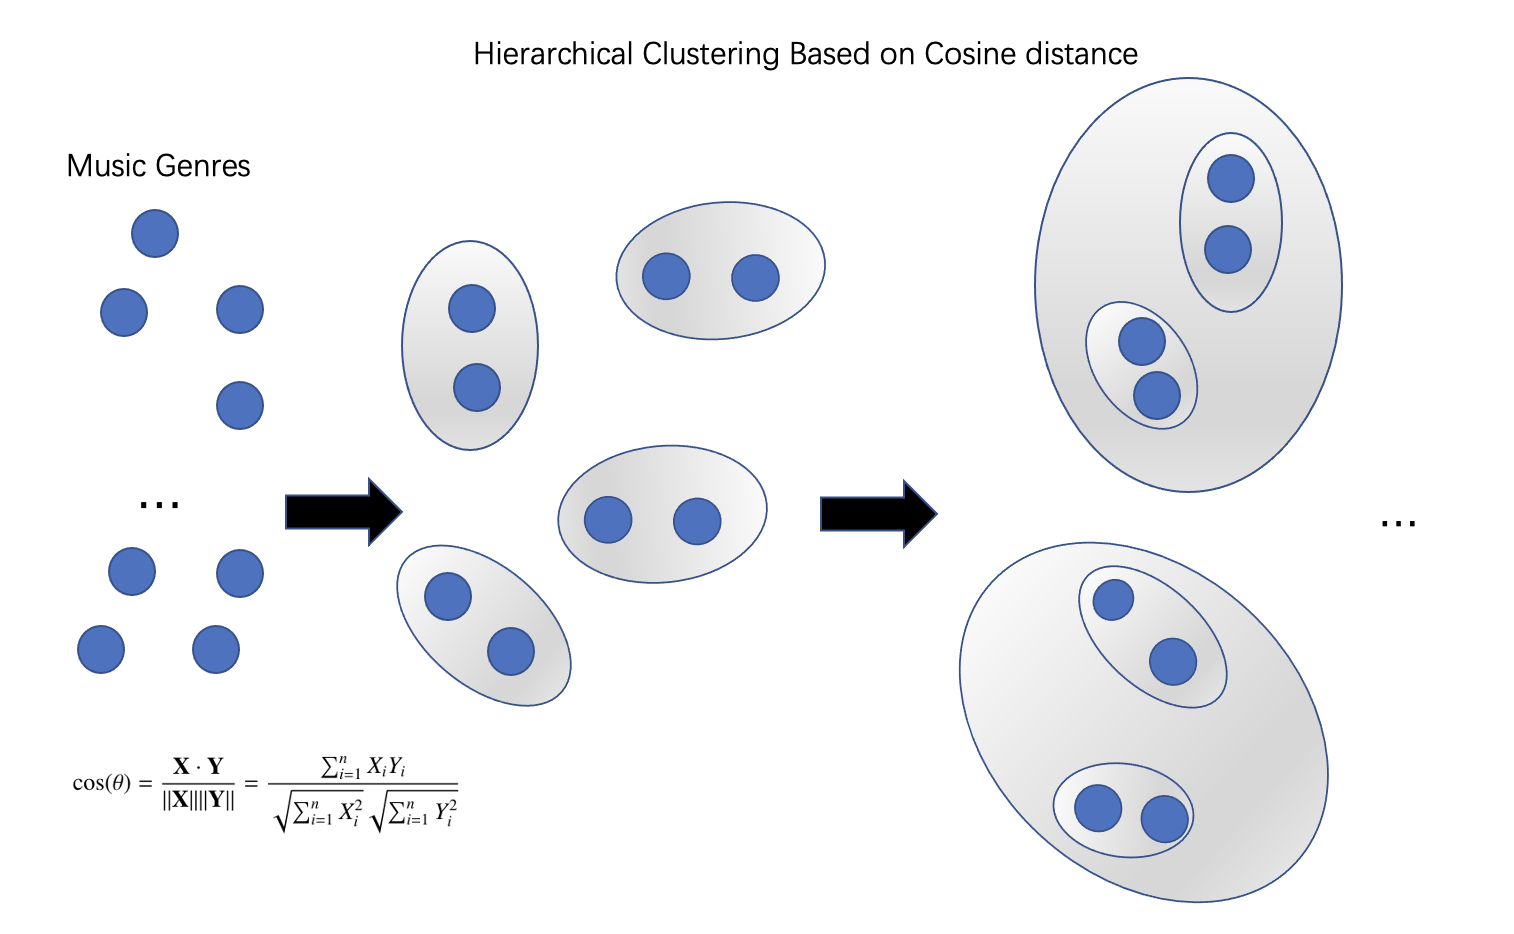
\includegraphics[width=8cm]{figures/Q2_hclurationale.png}
\label{hclusterrationale}
\caption{Rationale of Hierarchical Clustering}
\end{minipage}
\begin{minipage}[t]{0.48\textwidth}
\centering
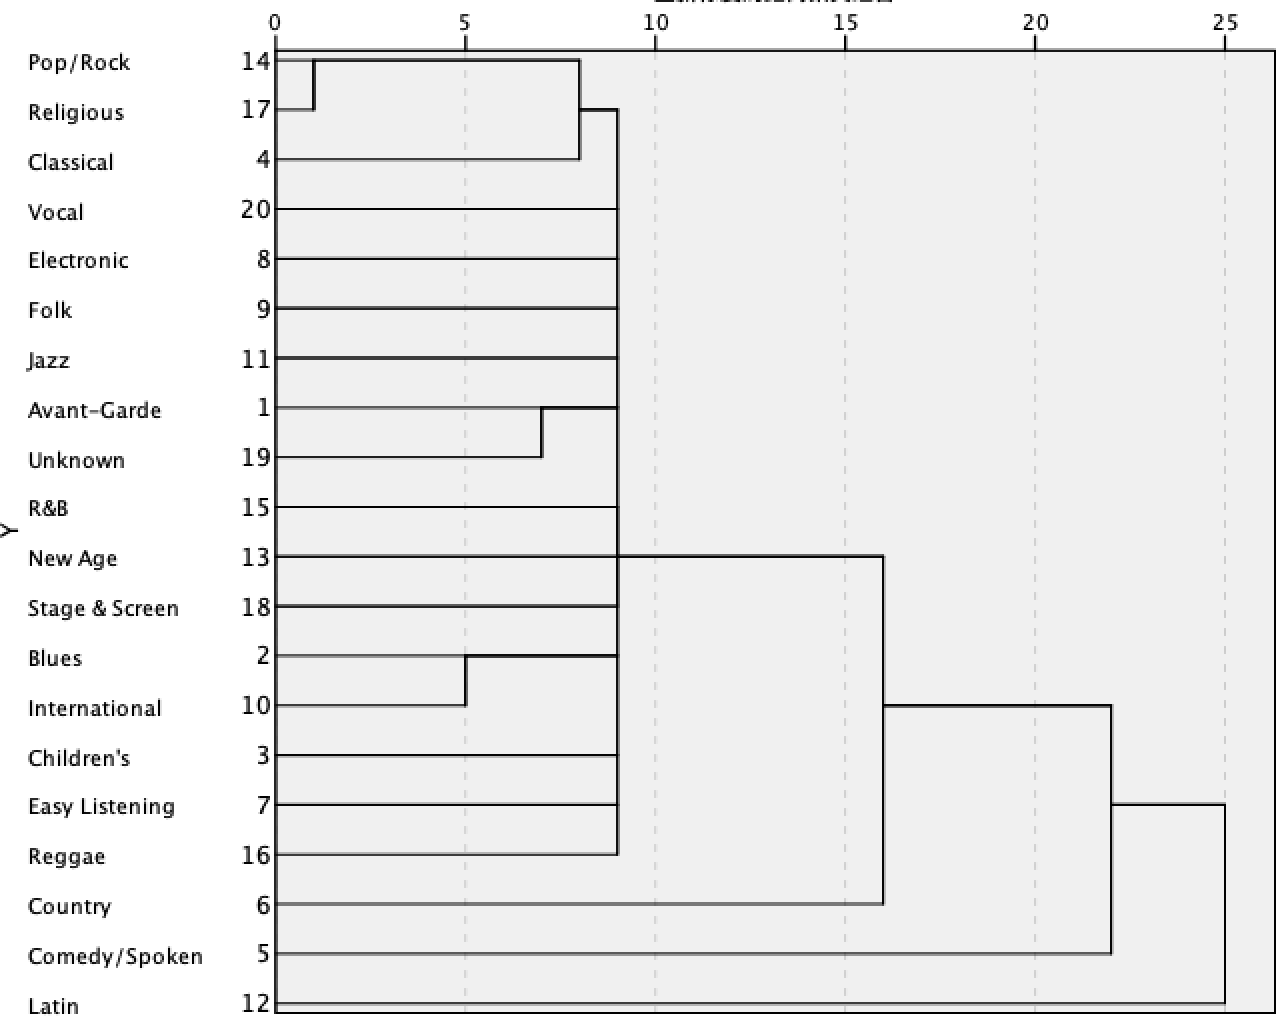
\includegraphics[width=8cm]{figures/Q2-hclustering.png}
\caption{Hierarchical Clustering Result}
\label{Hierarchical Clustering}
\end{minipage}
\end{figure}

The result from Figure \ref{Hierarchical Clustering} shows that Pop/Rock is has a closed relationship with the Religious, with distance ranging from 0 to 1, while the Latin music lies far away from other music genres, with relative distance up to 25, which is consistent with our common sense. However, in order to explore the music quantitatively without being affected by the subjective sense, we need to take the time into consideration. And the next section will explore that how artists or their corresponding genres change over time.

\section{Evolution of the Music Genres}

\subsection{Changes in the influencers and followers}
To examine the evolutionary and revolutionary trends of artists and genres, we do visualizations using line charts. 

Through the processing of the data in the \emph{influence\_data} data set, by calculating the number of influencers and followers in each genre and sorting by time, the music influence changing with time can be observed and determined the peak years in different fields based on the greatest number of new talents. 
\begin{figure}[H]
\label{fig:aa}
\small
\centering
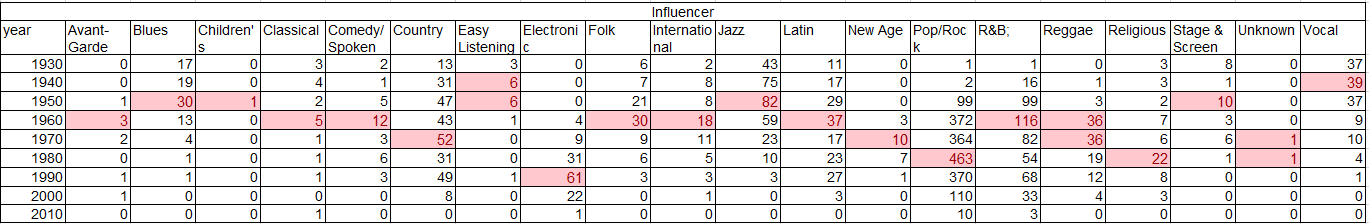
\includegraphics[width=12cm]{figures/Q1_influencer_data.PNG}
\caption{Number of influencers in different genres each year}
\label{influencer data}
\end{figure}

Figure \ref{influencer data} marks the greatest number of influencers. Each genre has one or two peak years. From the data in the above figure, we get the line chart in the left side below through analysis.
\begin{figure}[H]
\label{fig:aa}
\small
\centering
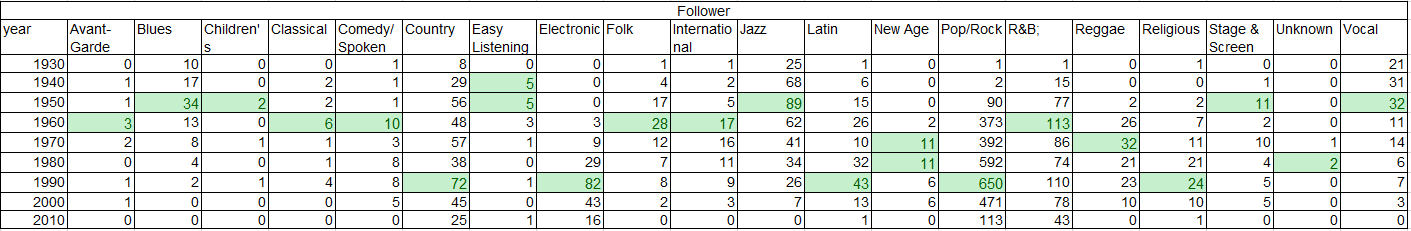
\includegraphics[width=12cm]{figures/Q1_follower_data.png}
\caption{Number of follower in different genres each year}
\label{follower data}
\end{figure}

Figure \ref{follower data} marks the greatest number of followers which indicates the new generation and flourish of each genre. From the data in the above figure, we get the line chart below in the right side.
\begin{figure}[H]
\centering
\subfigure[Line chart for influencers]{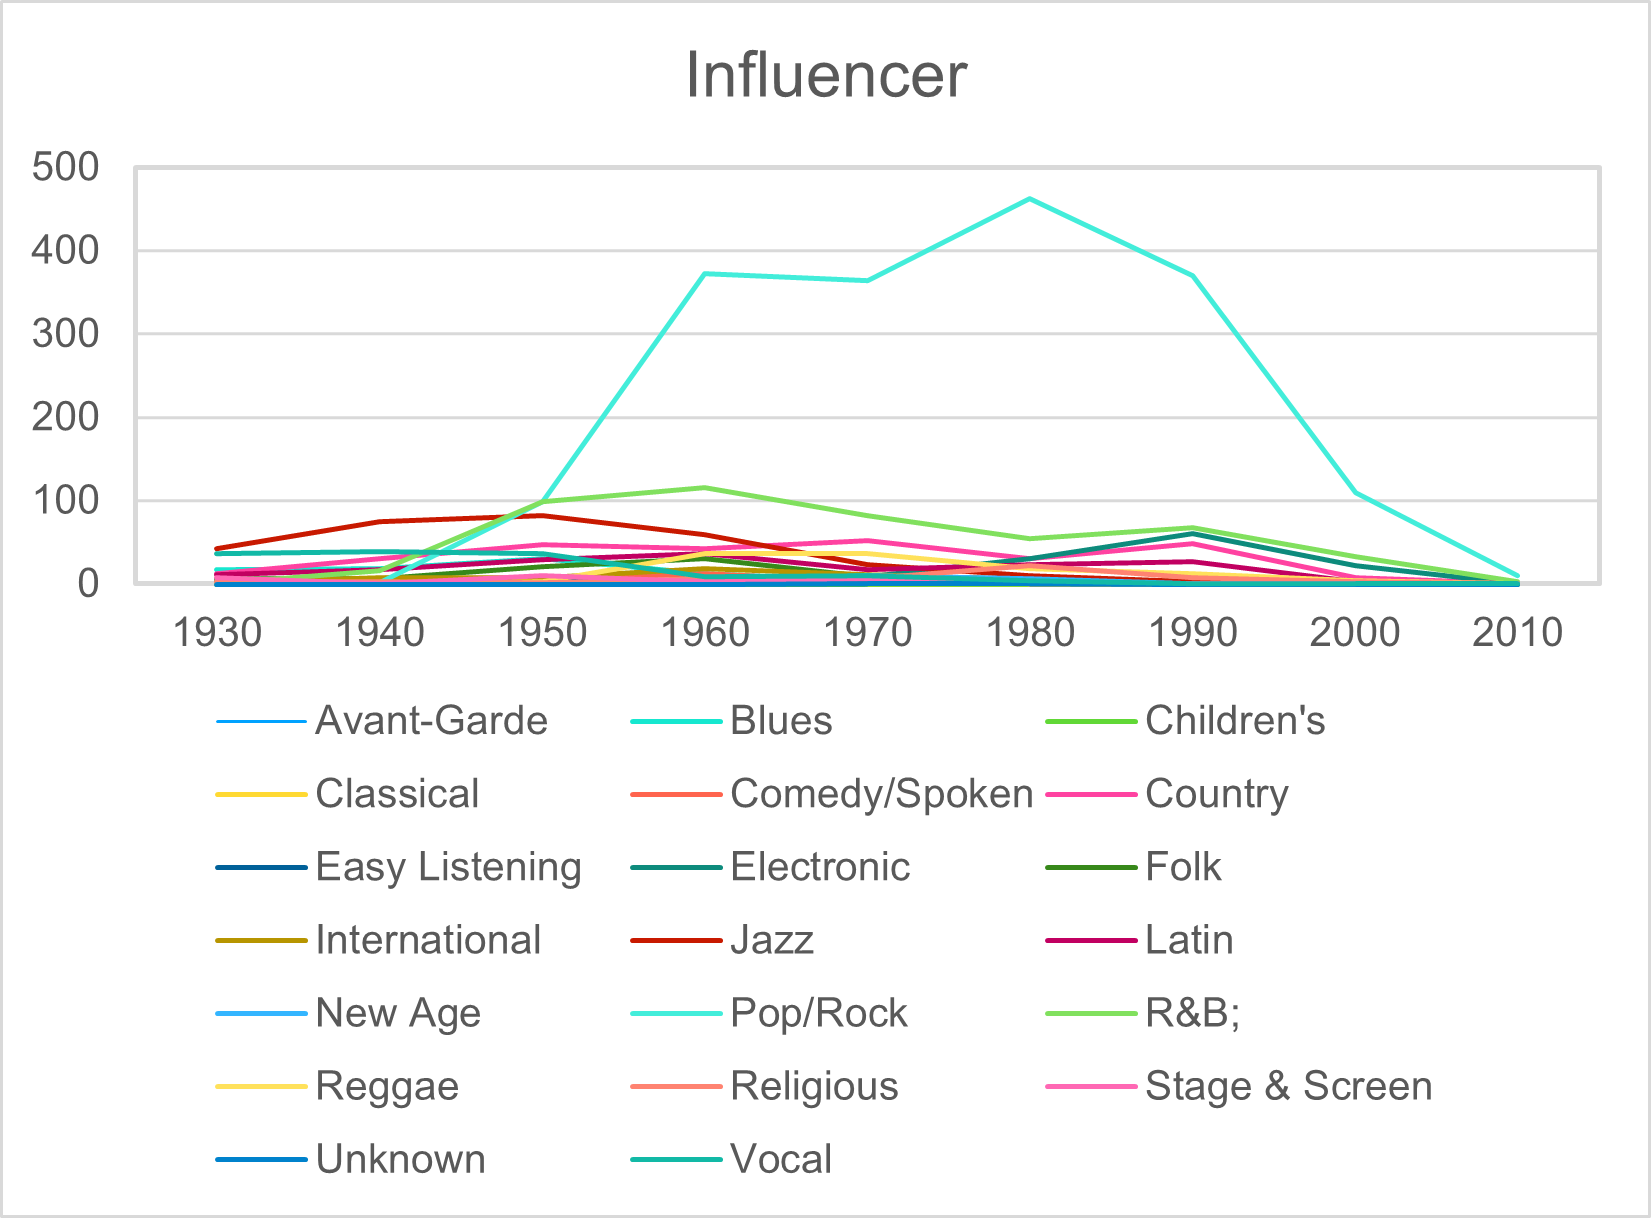
\includegraphics[width=6cm]{figures/Q1_influencer2.png}}
\subfigure[Line chart for followers]{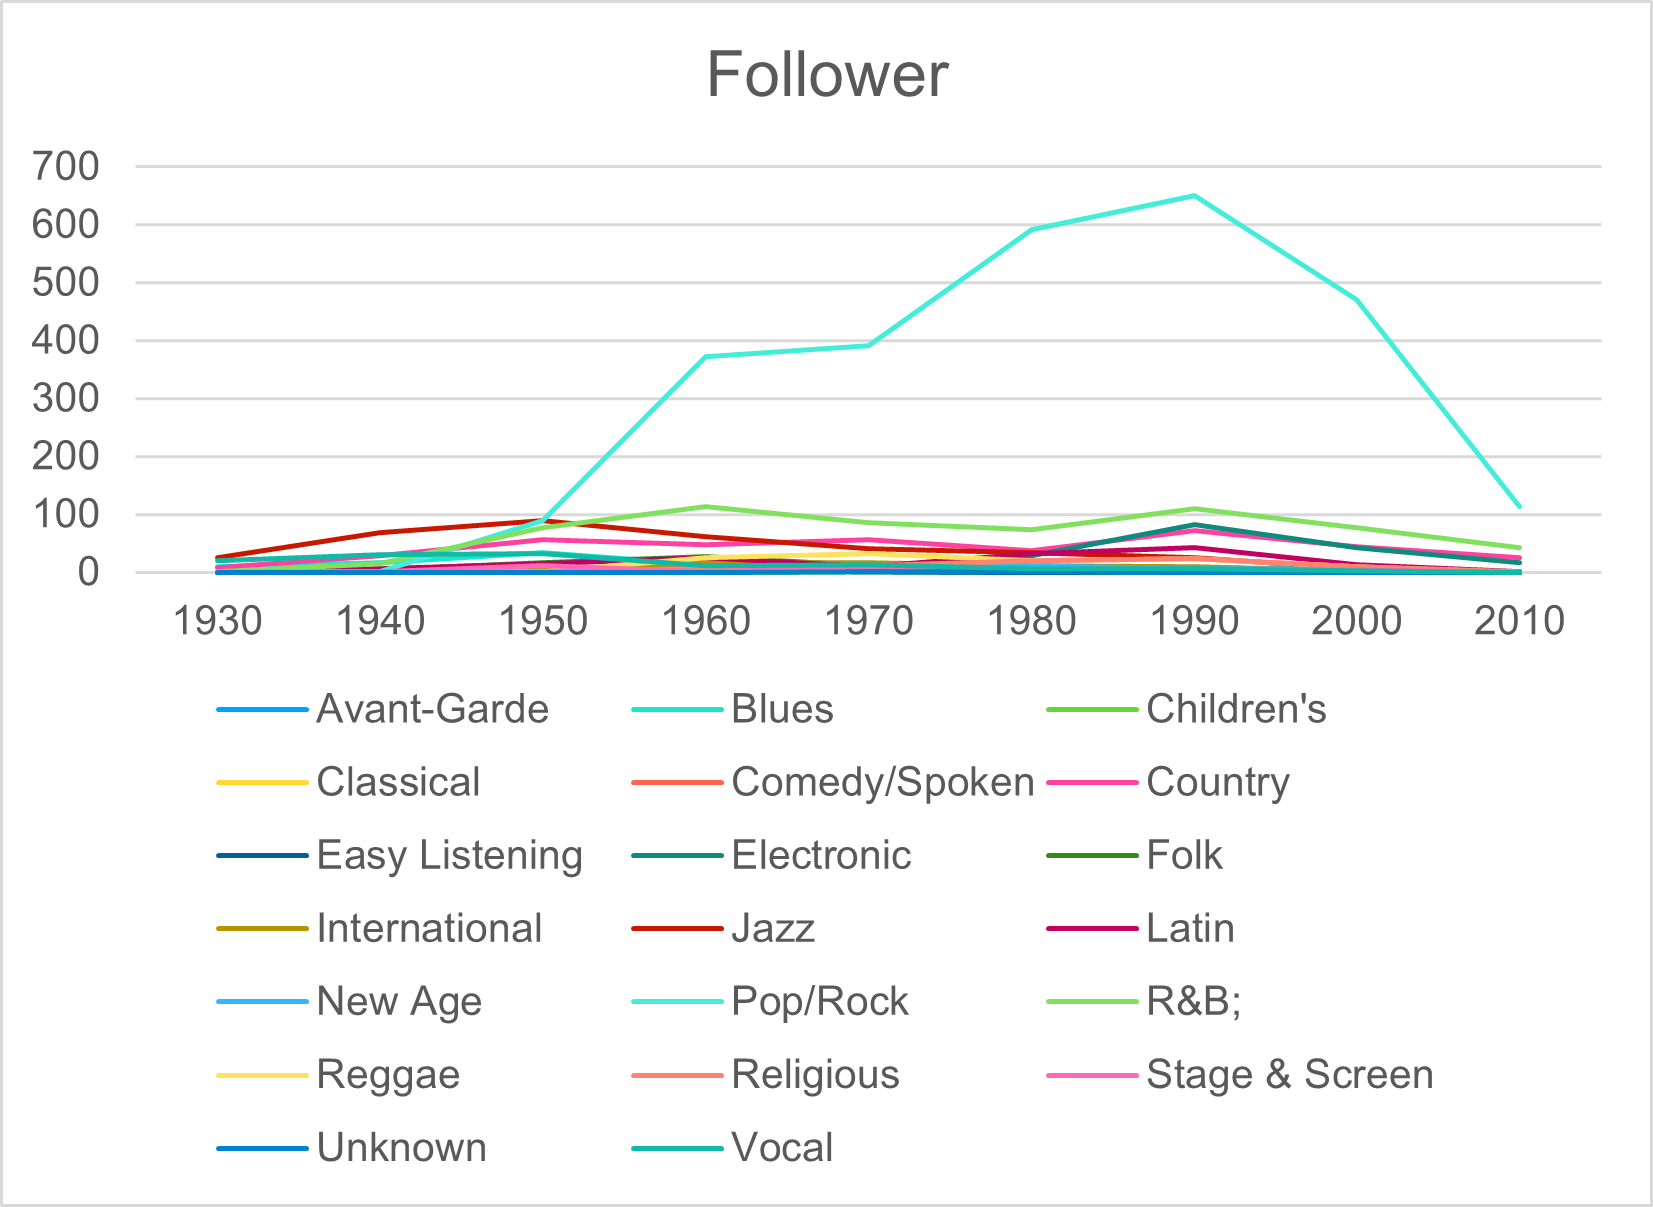
\includegraphics[width=6cm]{figures/Q1_follower2.png}}
\caption{Line chart for influencers and followers in different genres each year}
\label{line chart}
\end{figure}


From Figure \ref{line chart}, it can be seen that each field’s influencer and follower have a rise and fall time from 1930 to 2010. The change in the number of influencers will influence the variation of the follower. The influencer and follower almost change synchronously after comparing two pictures in Figure \ref{line chart}. 

The slopes in Figure \ref{line chart} indicate the developing speed of each field with time. When one field becomes hot, there are always some other fields fading. Most of the fields only spring up one or two decades. This may because many artists change their genres frequently with the stream. For those genres that have similarities or connections like Pop and R\&B, they could have similar change trends. In the figures above, they are kept in a relatively high number from 1960 to 1990.

\subsection{Changes in the full songs}
Combine with the \emph{full\_music\_data} data set, dividing different types of songs in their period and counting the total number, Figure \ref{full table} gives the total amount of songs and Figure \ref{full songs} shows the trend of each genre, which almost meets the changing trend above. 
\begin{figure}[H]
\label{fig:aa}
\small
\centering
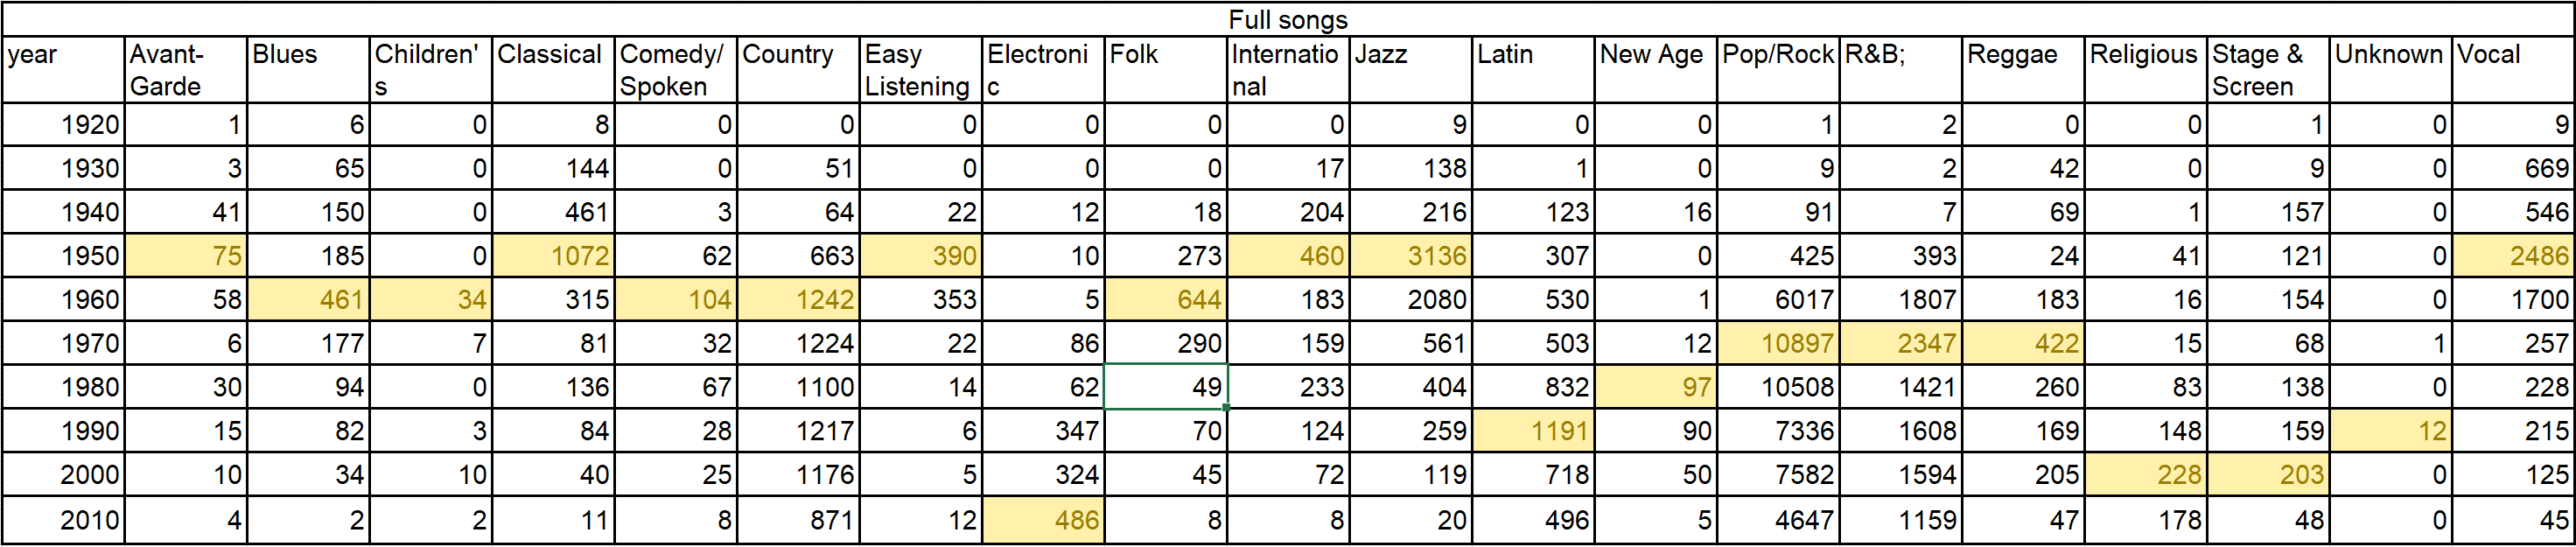
\includegraphics[width=12cm]{figures/Q3_Full_table.png}
\caption{Full songs in different genres each year}
\label{full table}
\end{figure}

Figure \ref{full songs} also shows that when one field becomes popular, other fields will have fewer songs, which has similarities with the decreasing number of artists. This finally leads to the decline of one genre. 
\begin{figure}[H]
\label{fig:aa}
\small
\centering
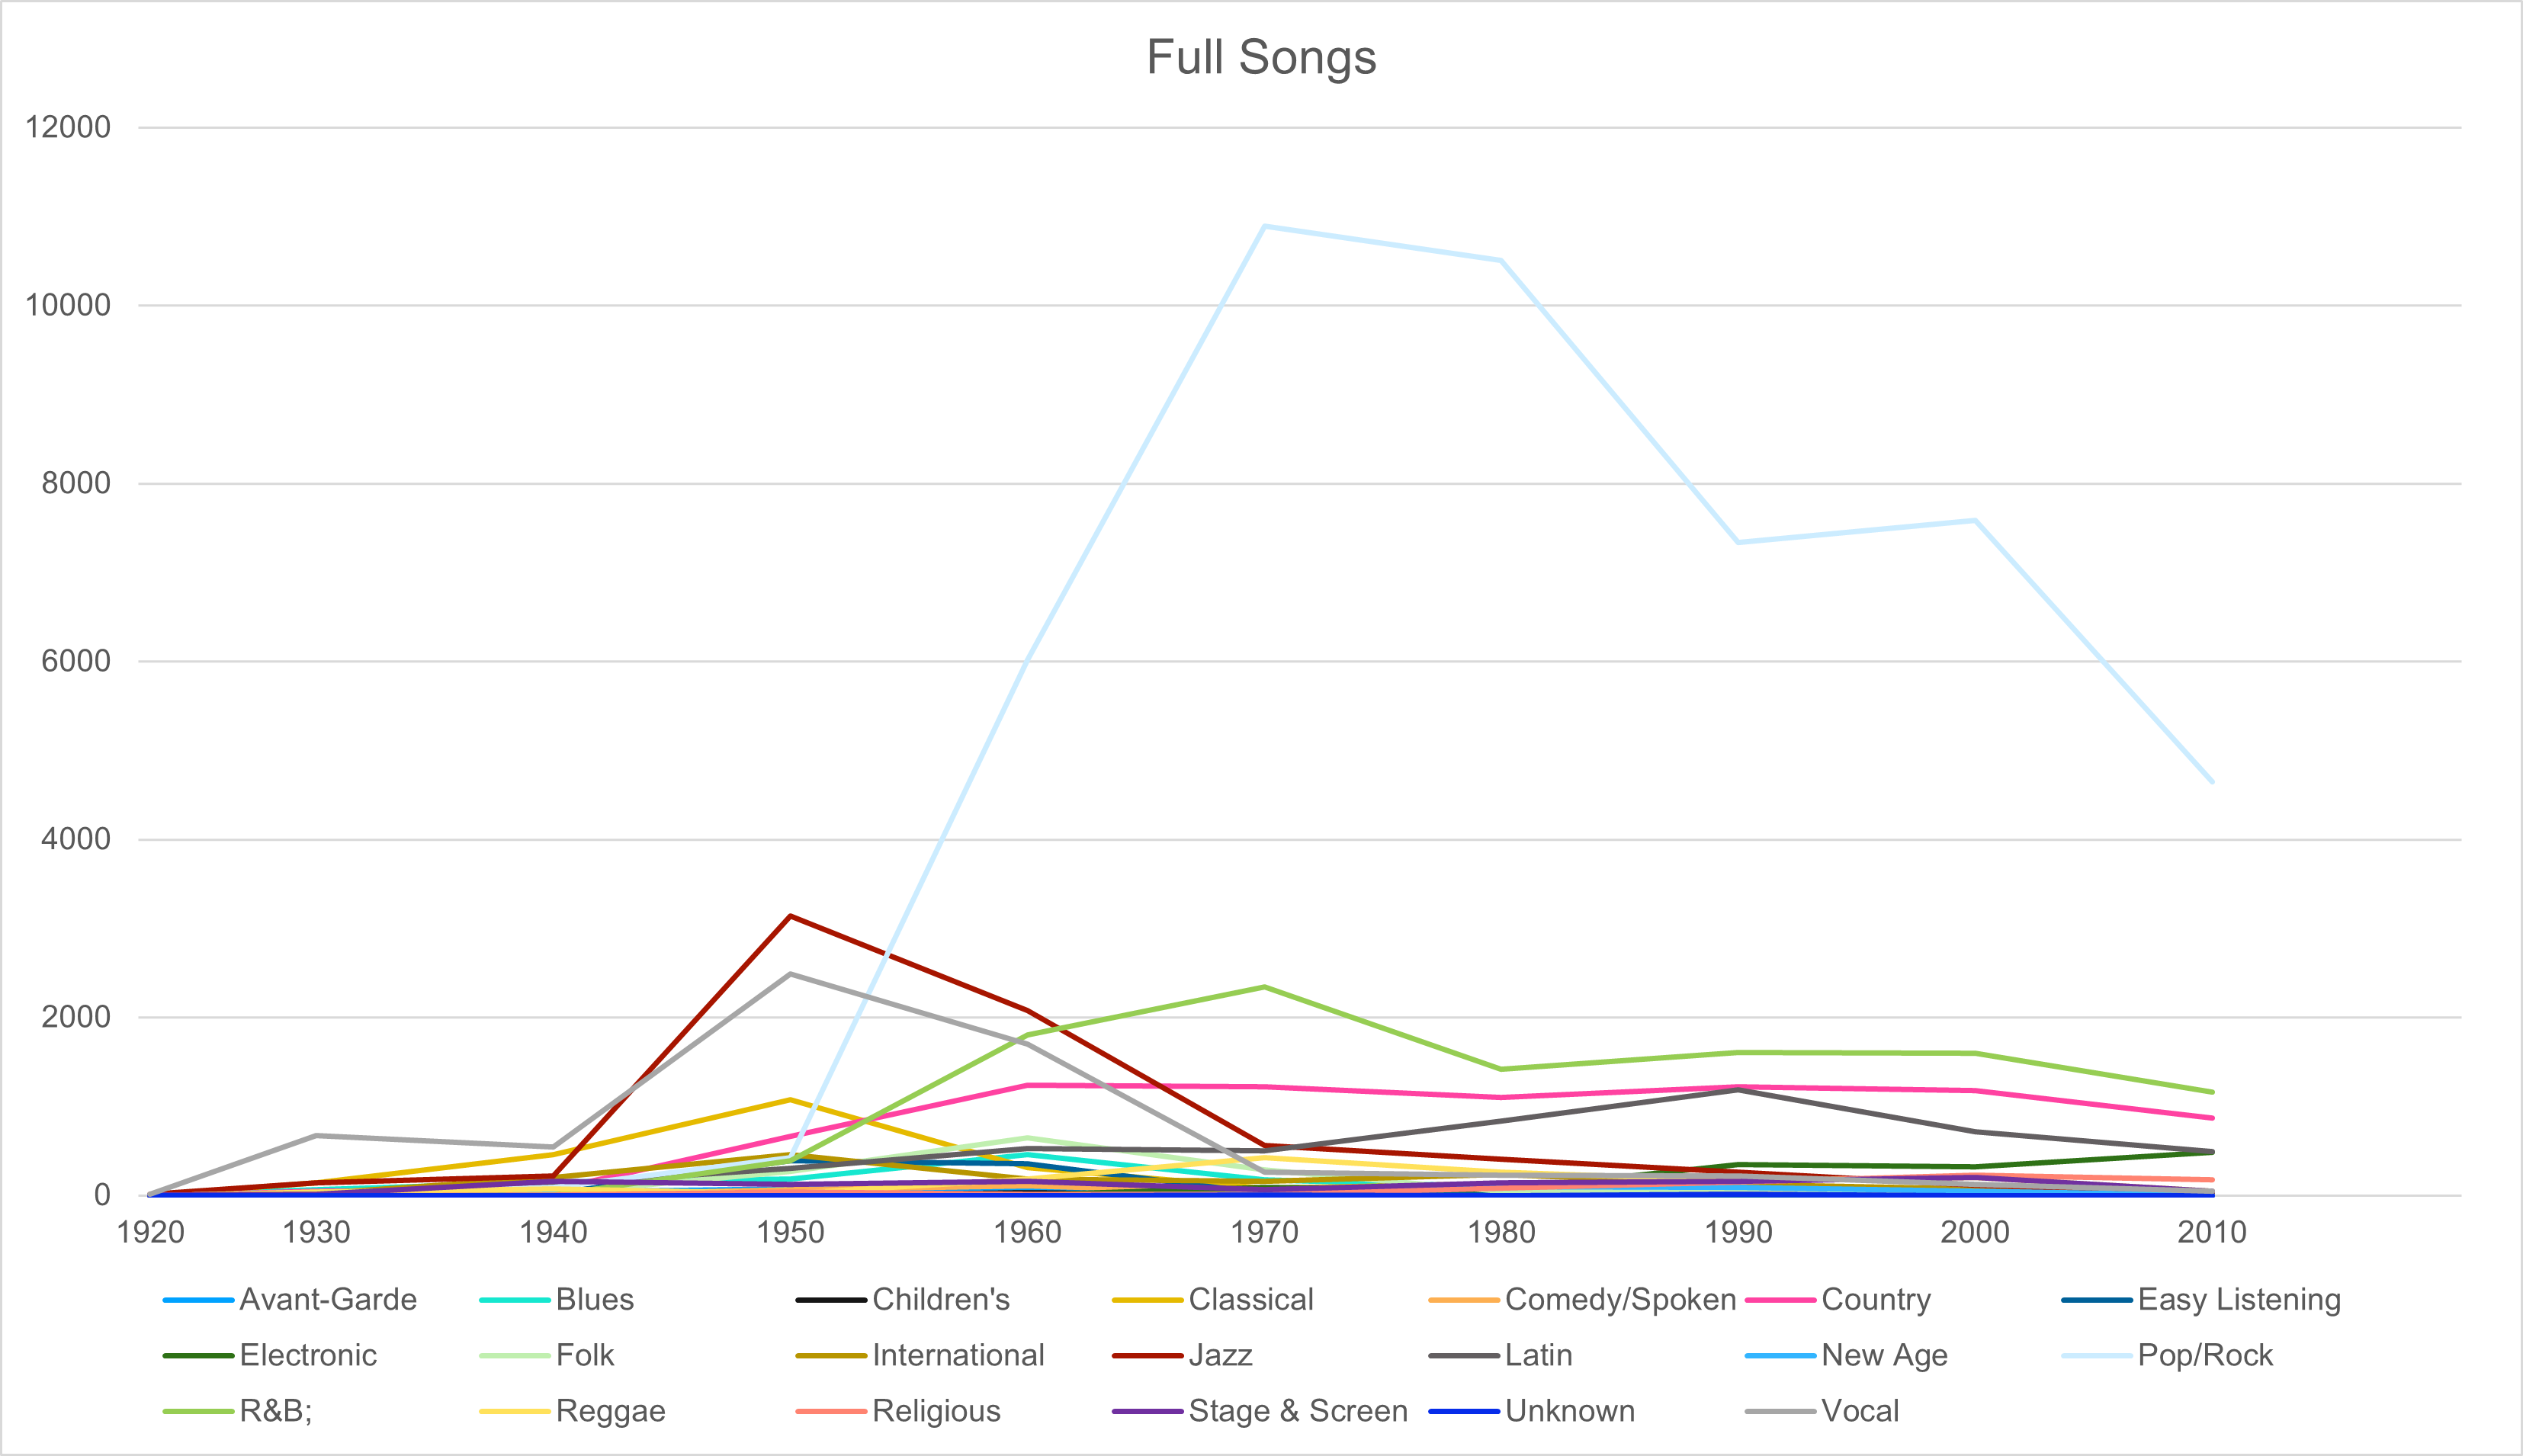
\includegraphics[width=12cm]{figures/Q3_Full_song.png}
\caption{Number of songs in different genres each year}
\label{full songs}
\end{figure}

\subsection{Changes in Pop/Rock Over time}
Looking at the certain genre, we chose the distinct one, which is Pop/Rock. The Pop/Rock music has a sharp rising time of artists around 1950 to 1990 with a peak in 1990 and falls down after that. From Table \ref{Top 6 Most Influential Artists}, we know that \emph{The Beatles} has the most followers in Pop/Rock and start activation in 1960. From the data set, they released 120 songs in 1967, which is the year with the most releases and their most popular song is released in 1969. According to Table \ref{Top 1 Most Influential Artist Each Year}, between 1960 to 2000, the most influential artists belong to Pop/Rock. This may lead to the rising of Pop/Rock during that time.

Using the \emph{full\_music\_data} data set, after standardizing all data into 0 to 1 scale, we plot the change of all characteristics with time in Figure \ref{Pop}.
\begin{figure}[H]
\label{fig:aa}
\small
\centering
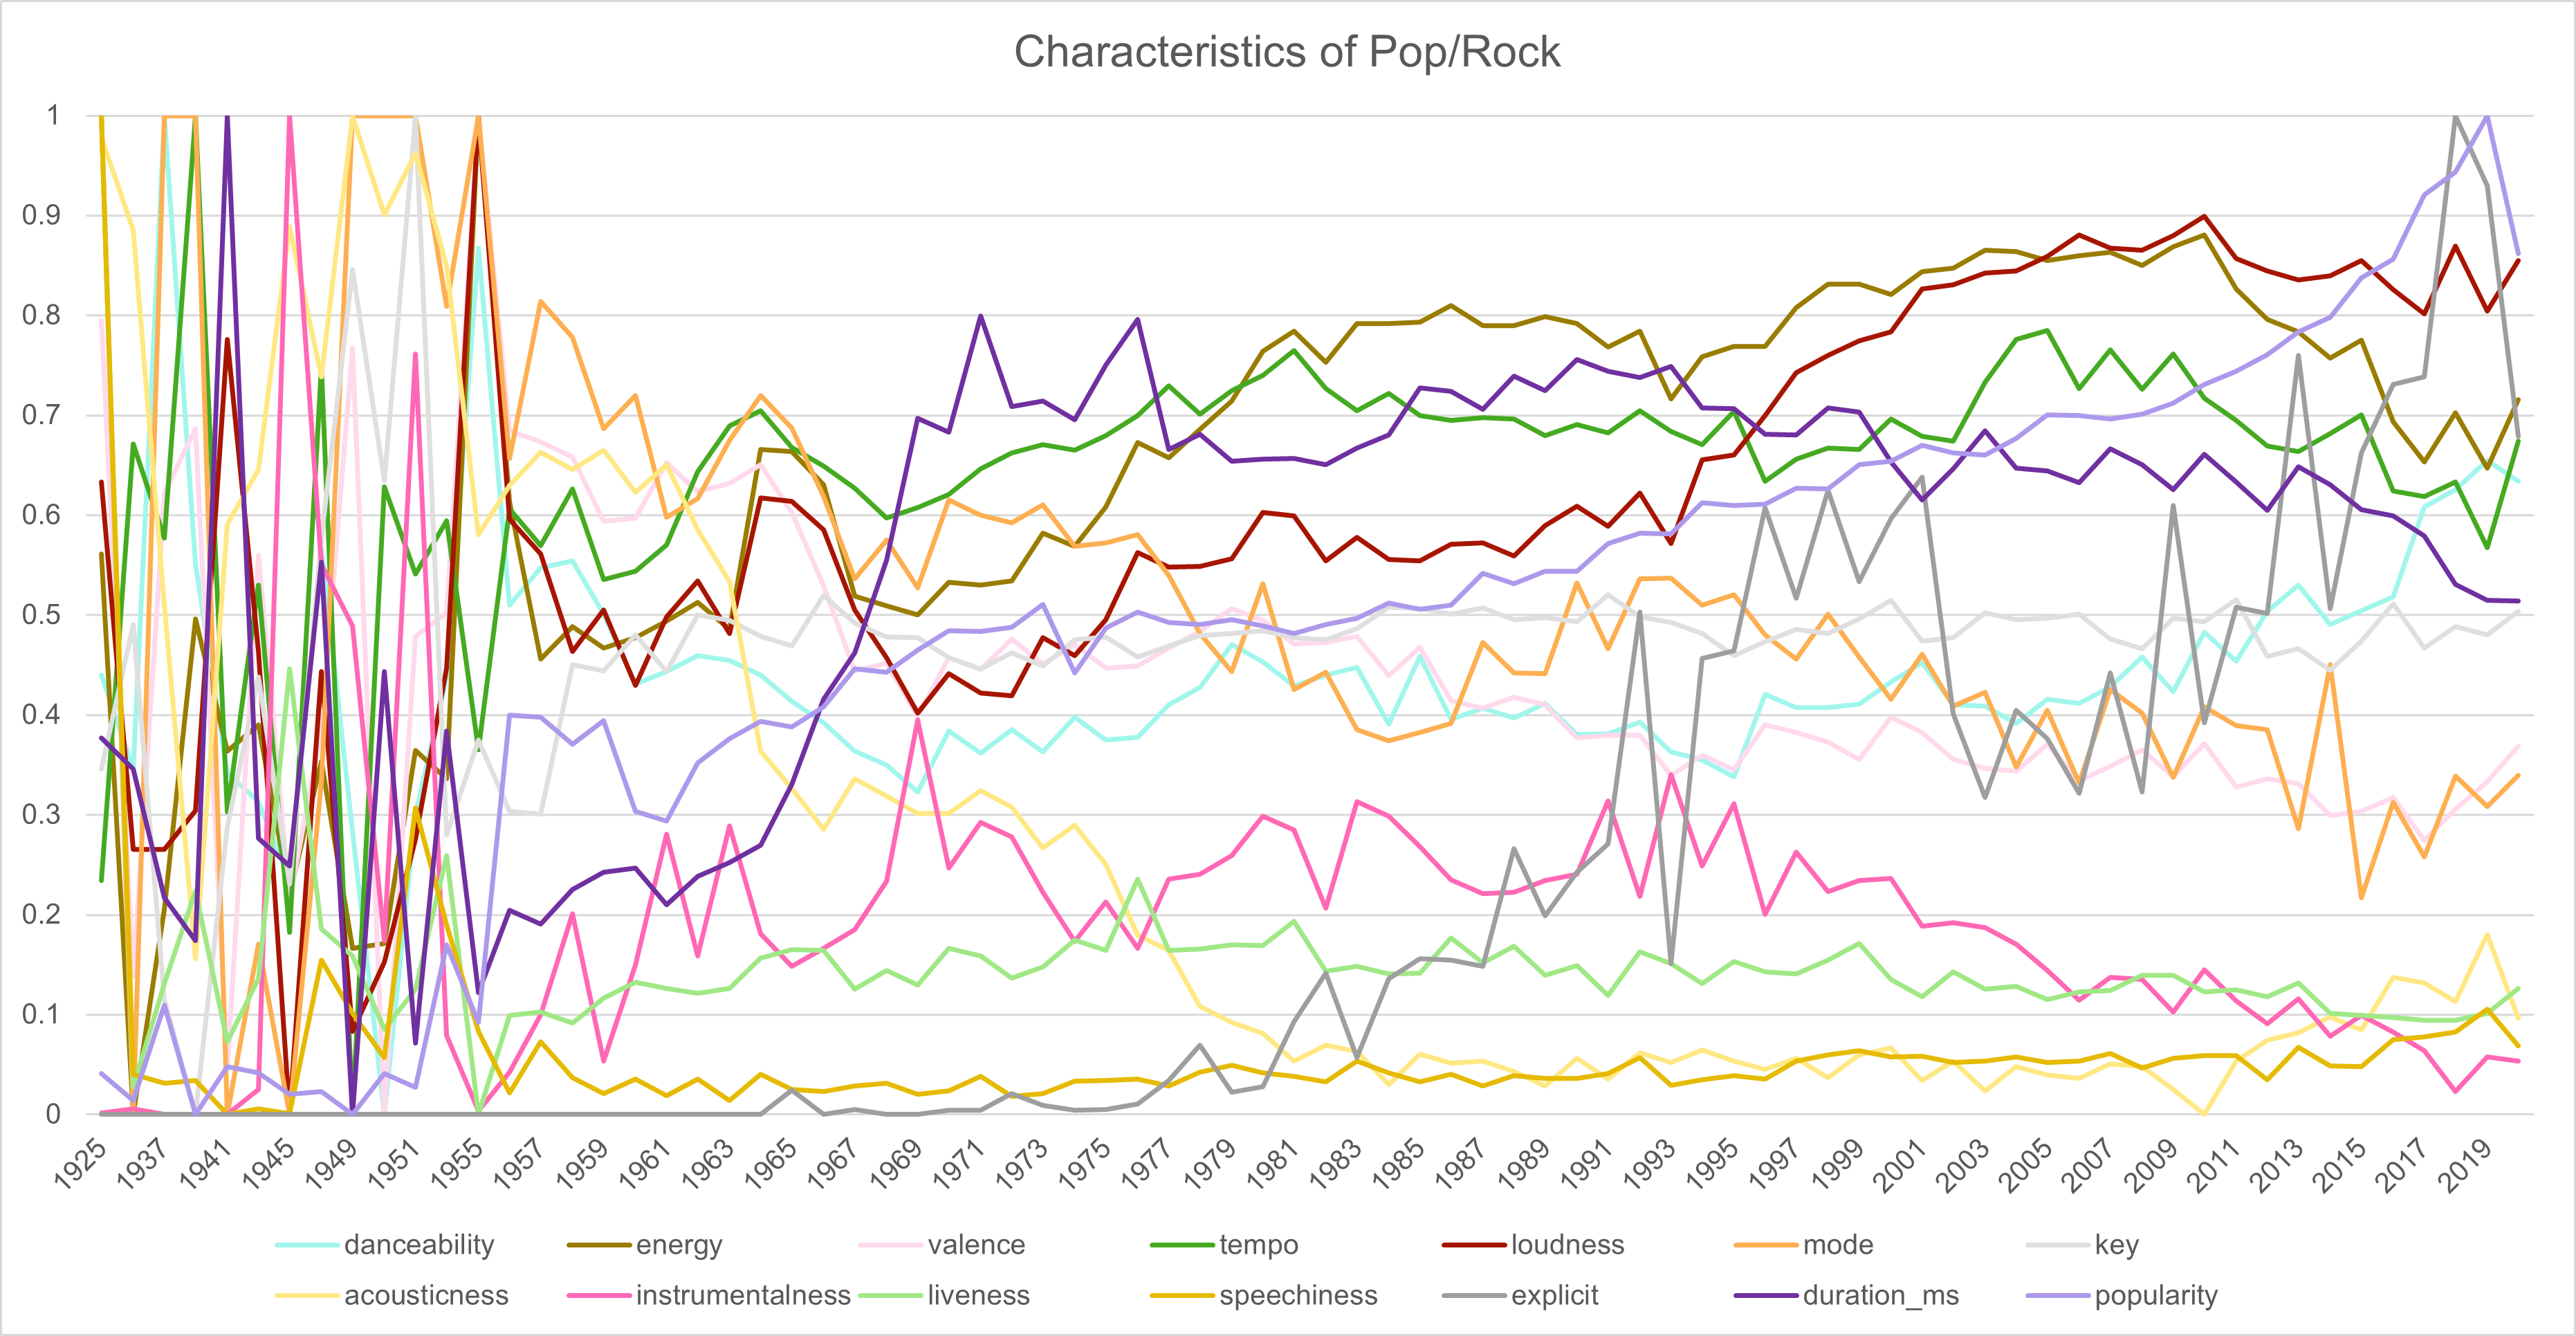
\includegraphics[width=12cm]{figures/Q3_POP.png}
\caption{Characteristics of Pop/Rock}
\label{Pop} 
\end{figure}

It can be seen that the general tendency of popularity is increasing. This indicates the rising position of Pop/Rock in history. Although the number of the full song has decreased, it still more than other genres, which meets the previous result.
\begin{figure}[H]
\centering
\subfigure[Line chart for Pop/Rock]{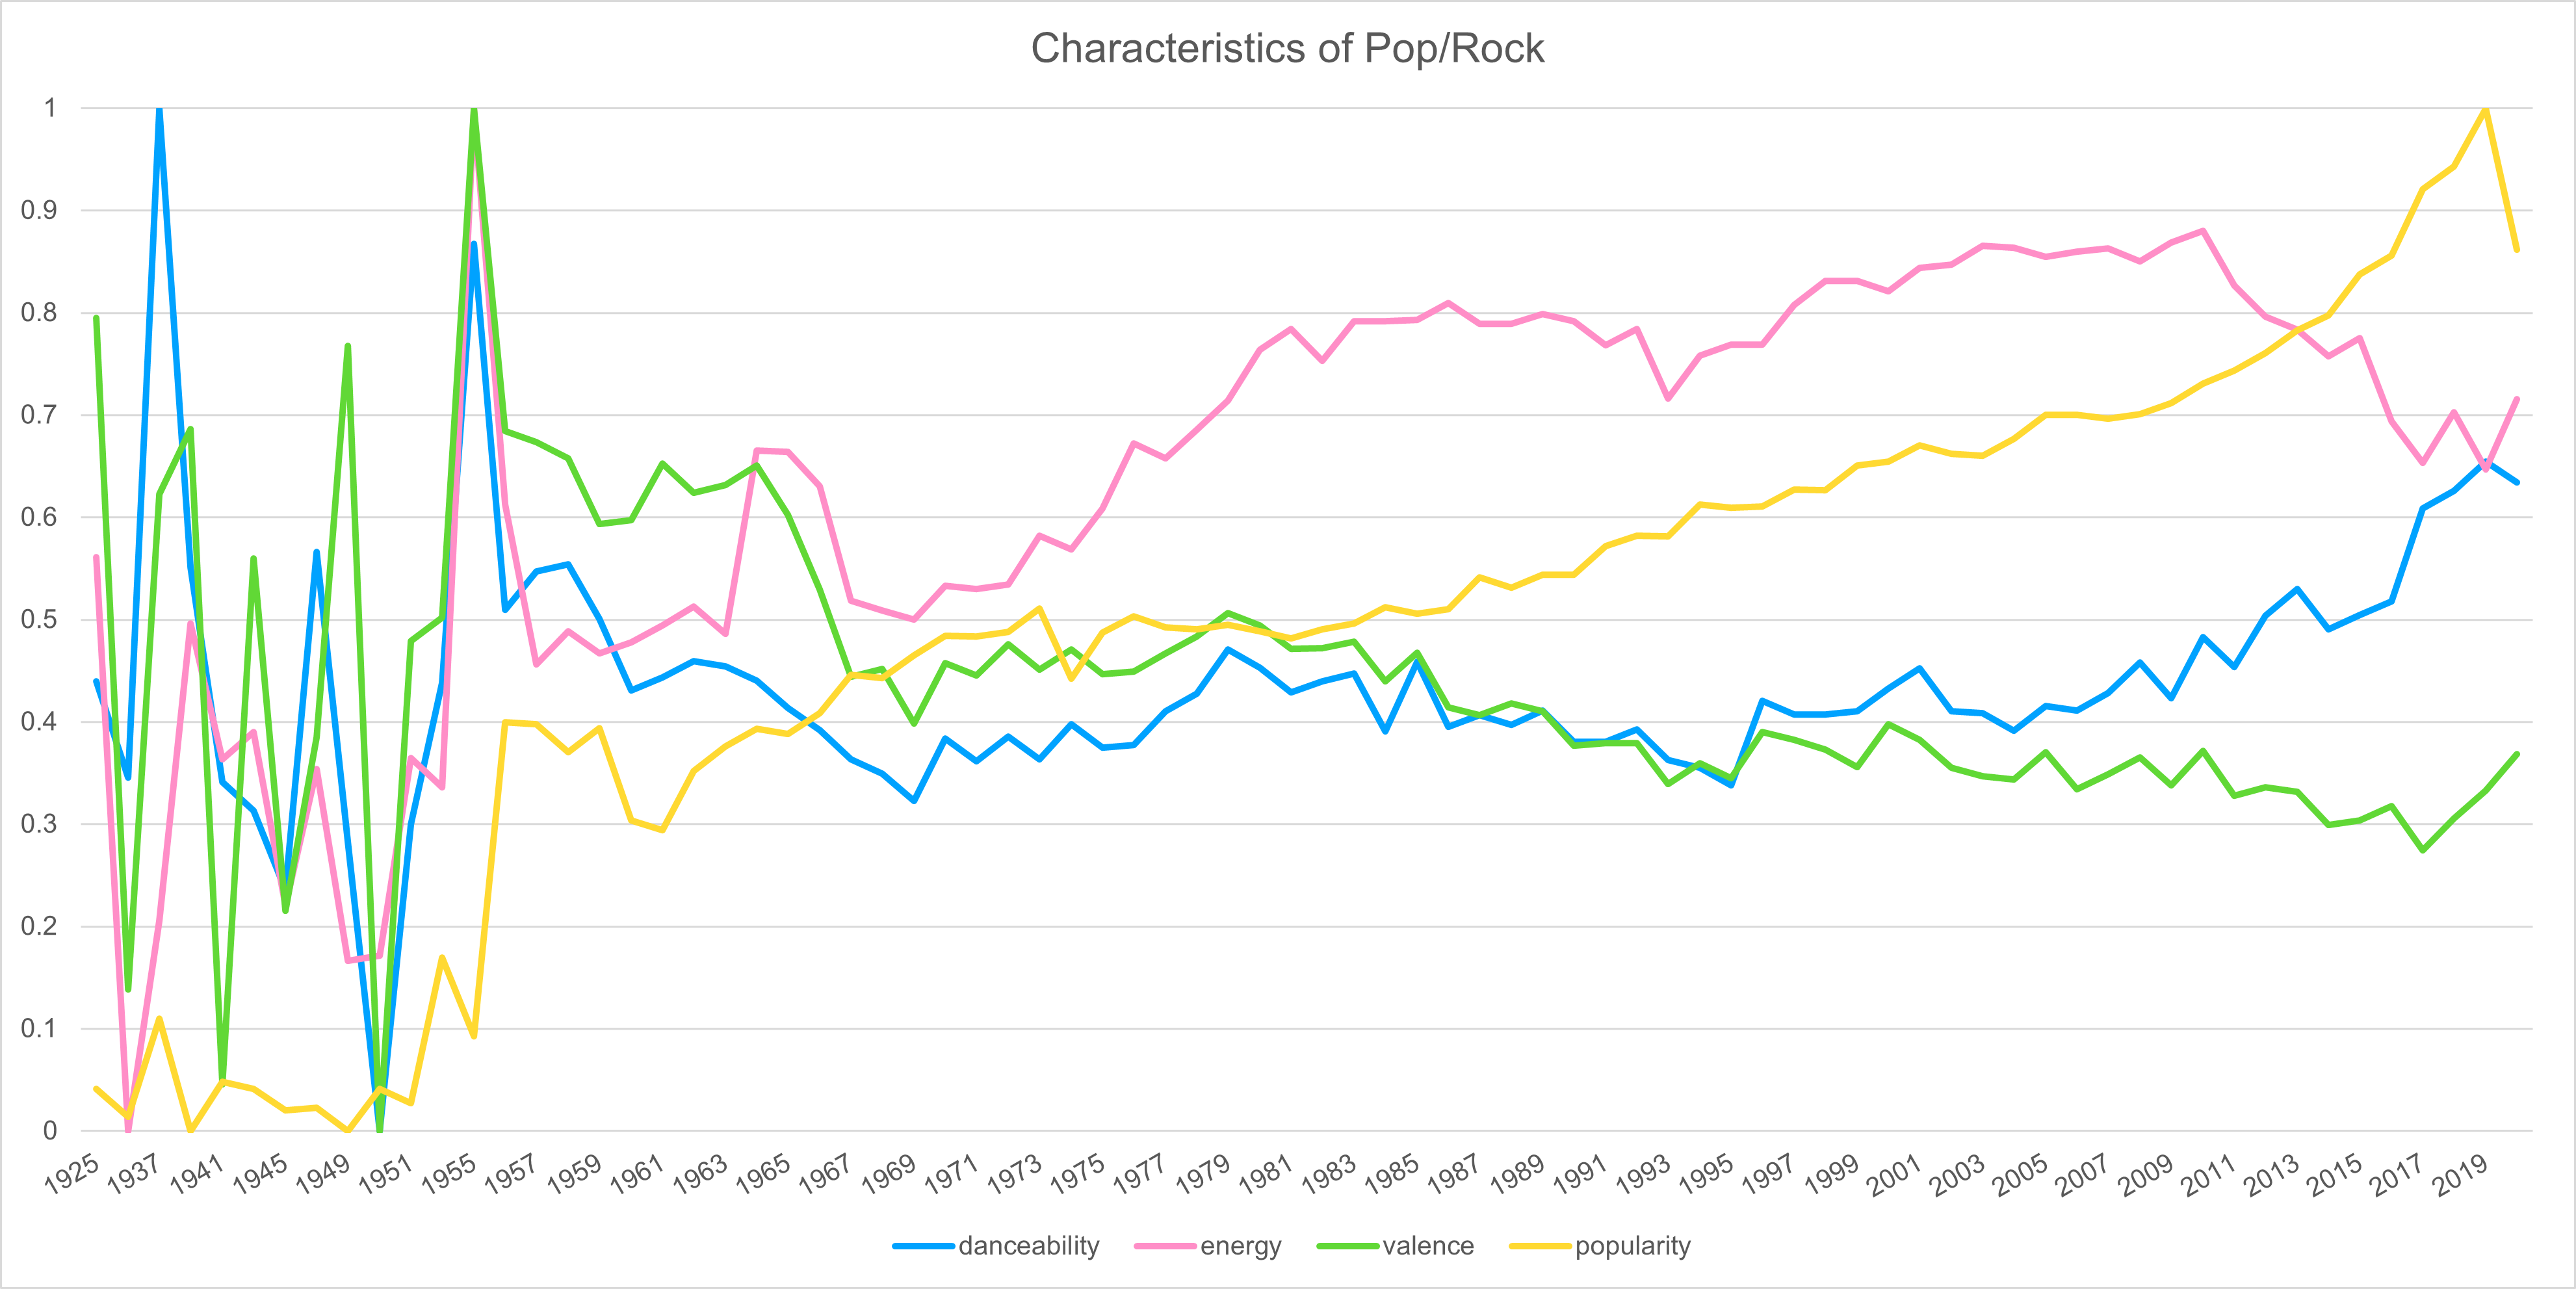
\includegraphics[width=6cm]{figures/Q3_1.png}}
\subfigure[Line chart for The Beatles]{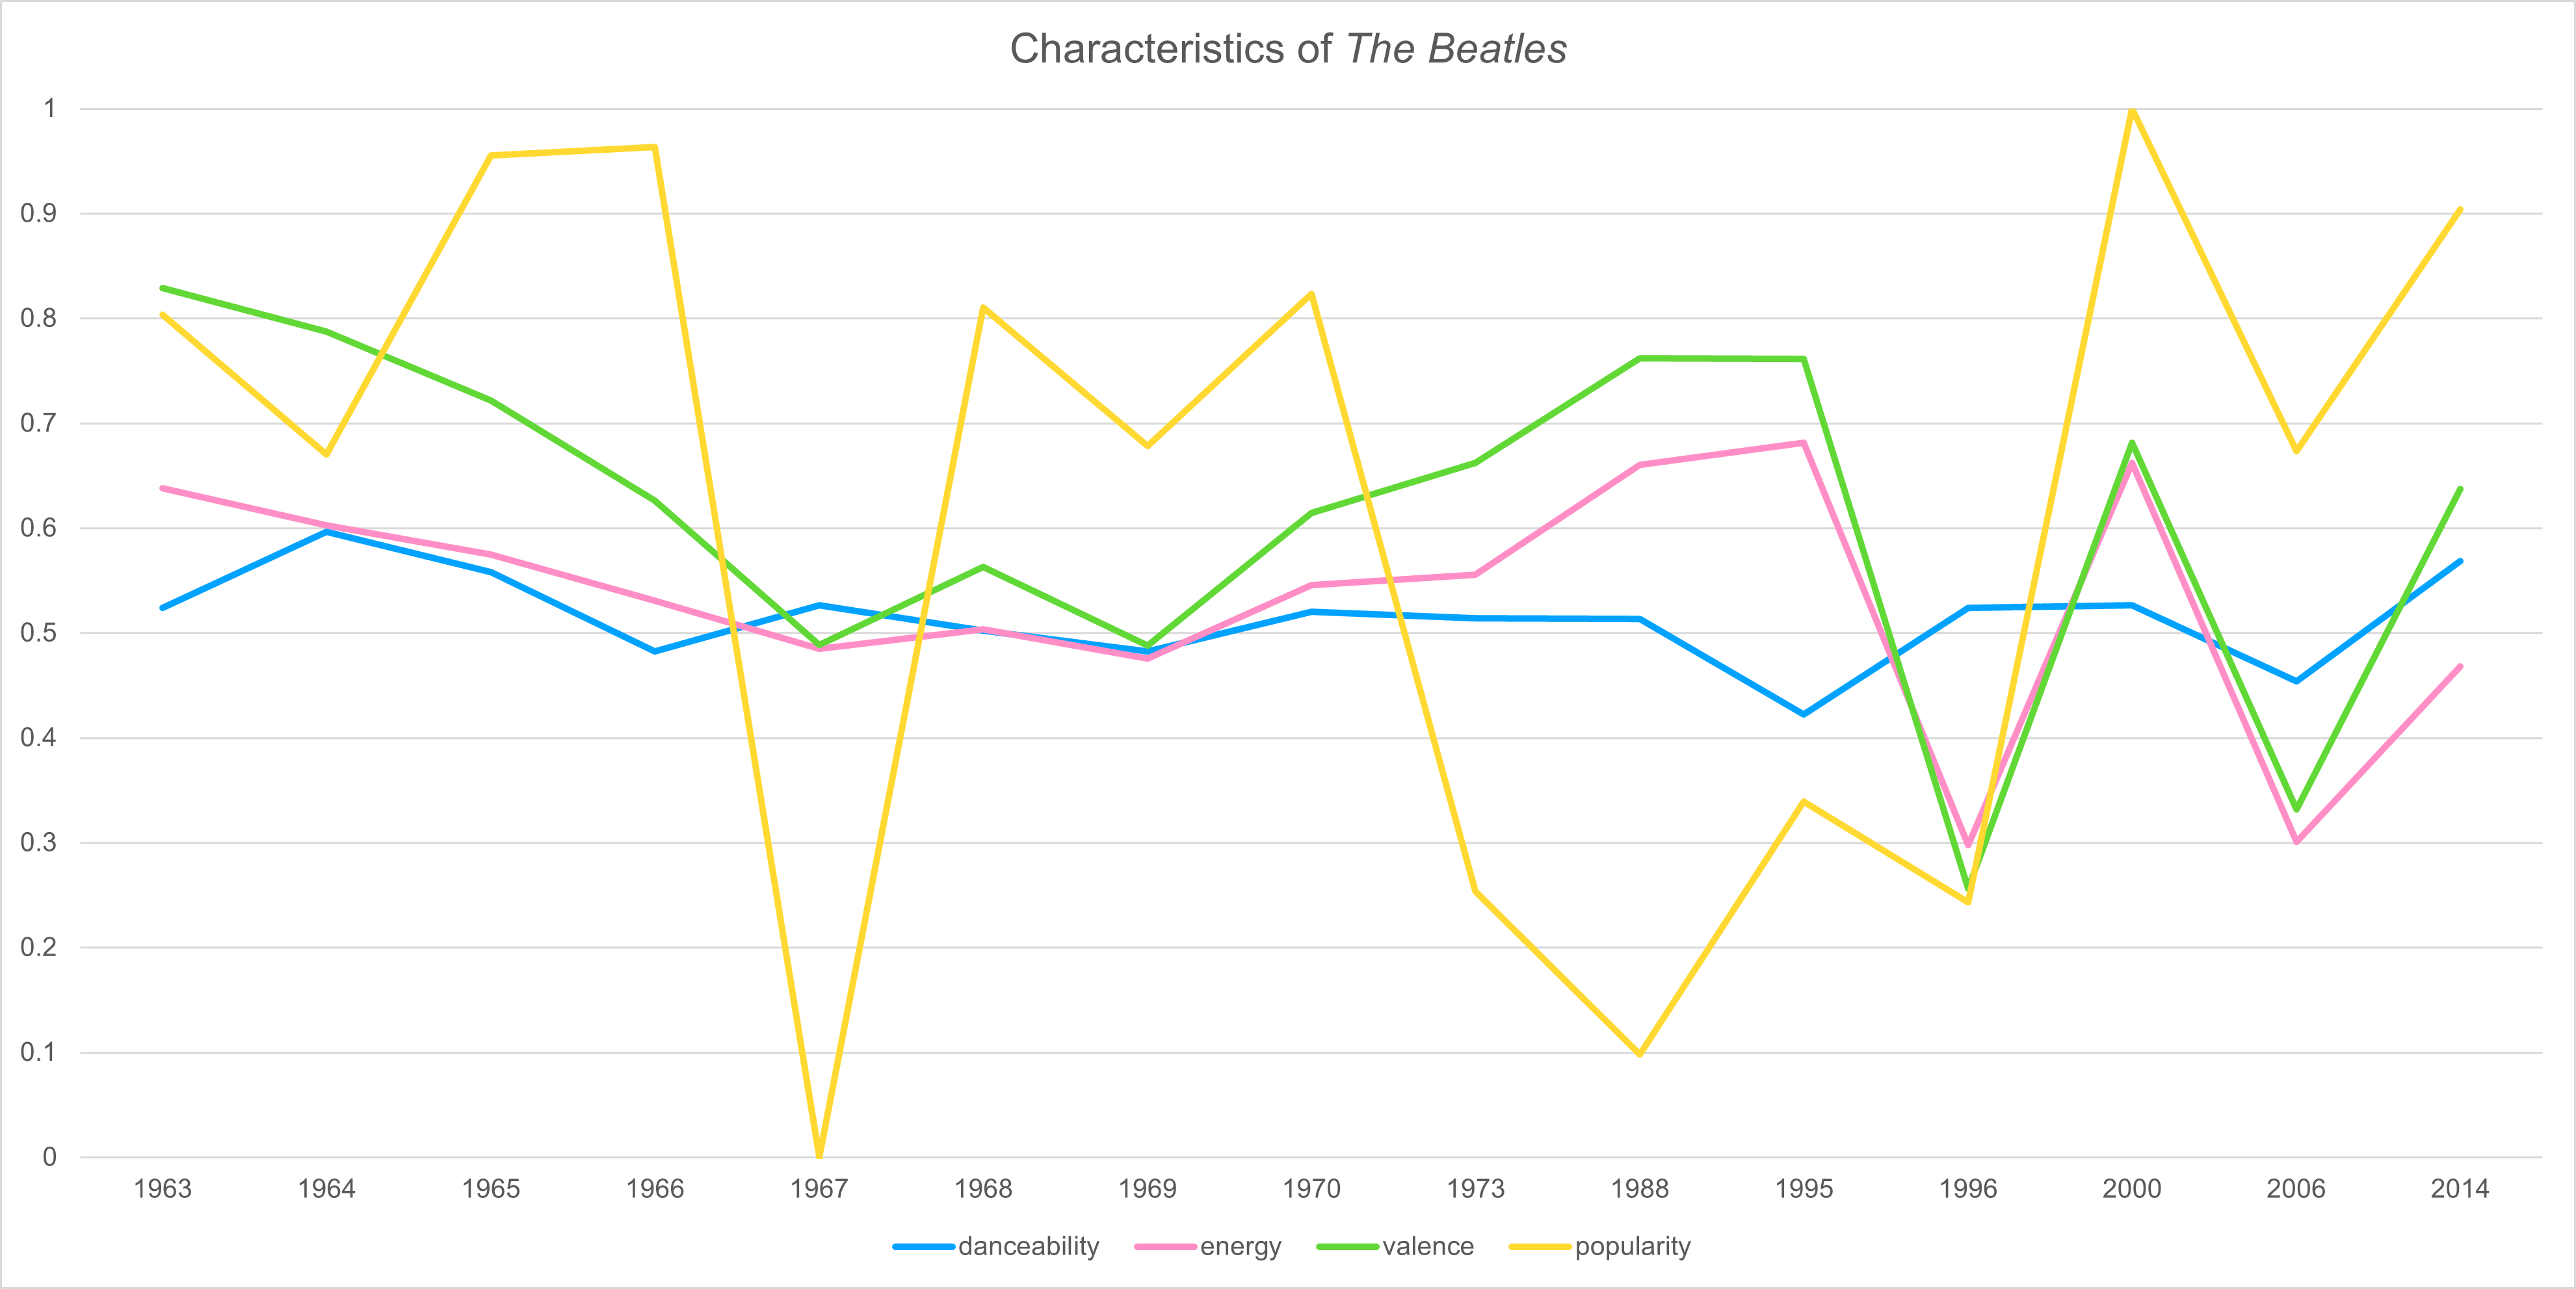
\includegraphics[width=6cm]{figures/Q3_2.png}}
\caption{The characteristics between one genre and artist}
\label{characteristics}
\end{figure}

For Pop/Rock music, we further focus on \textbf{danceability, energy, valence and popularity} in the whole field and the most influential artists with the time change. From the figure above, we find that the change of the single artist is not the same with the whole genre. 

\textbf{Every musician might have a trough period and popular season, while the whole area may only have a small variation due to their changes}. The characteristics of \emph{The Beatles} keep almost the same from it began. After the 1960s, Pop/Rock’s energy slowly grows until 2010. Then it falls down. The danceability and valence tend to be stable during this period. However, every genre will experience the boom goes to the bust, then slowly from the bust to the second boom with evolutions over time.

\section{Strengths and weaknesses}
\subsection{Strengths}
\begin{itemize}
    \item Our model can be widely used in engineering, management, social science and other related fields, especially interdisciplinary frontier research.
    \item It is an innovative use of the features of different music genres when analyzing the similarity.
    \item The value of modularity greater than 0.44 indicates a certain degree of modularization had reached by the network diagram. We get 0.7030, 0.6950, 0.6180, 0.5260, 0.6060, 0.6570, 0.7180, 0.8990 and 0.9000 for each network diagram (in order of years from 1930 to 2010), which shows our network diagram is significant.
    \item This model is especially suitable for mining a large amount of information from a complex system. Multidimensional problems would be solved by our model as well.
    \item Valuable information could be found by analyzing the time evolution along with the network model.
\end{itemize}
\subsection{Weaknesses}
\begin{itemize}
    \item There are many ways to measure the similarity, perhaps the cosine distance is not the best choice since it only justifies the direction but not the magnitude.
    \item Singular values can make a big difference for hierarchical clustering and the data are likely to be clustered in chains by mistake.
    \item The assumption that the average level of features could represent the whole level of a music genre might fail so that our model precision could be affected.
    \item Perhaps the time unit (year) is too long since the technological progression would make a difference in the short term.
\end{itemize}
\section{Model Extension}
Our model could be applied to many areas, such as social media networks, online shopping investigation and linguistics.
Let's take social media as an example. It is widely known that social media has a basic function showing the following and followers, which is almost the same as the followers and influencers in our music model. Based on this, we could build a network model to capture \textbf{how valuable information transfers among users, which could bring our attention to the scenes of major events around the world}.
\section{Conclusions}
\begin{itemize}
\item  The parameter "number of edges" indicates ‘music influence’ in the network. Different artists have a different number of edges, the more number of edges an artist has, the more influential the artist is. The "music influence" reveals that an artist's composition is influenced by another or several artists' compositions. In another word, artists' compositions are influenced by each other. For instance, the most influential artist \emph{"The Beatles"} from 1930 to 2010. They have the most mutual influencers (influencers + followers), so the node representing \emph{\textbf{"The Beatles"}} has the most complicated edges.

\item The \textbf{Pop/Rock, R\&B, and Religious} share a very closed relationship with each other, and the coefficient between the Pop/Rock and Religious is up to 0.8473, which is a very high level. 

\item The characteristic which could distinguish a genre is \textbf{speechiness}. Songs that have a large value in speechiness could be more likely the genre of Comedy/Spoken. Pop/Rock always has a higher value in instrumentalness and energy. And the genre’s popularity changes over time due to their characteristics’ change and the influencer's and follower’s variation in different fields. 

\item It is true that the ‘influencers’ actually affect the music created by the followers. For example, \emph{\textbf{David Bowie}}, who is a follower of \emph{"The Beatles"} in the Pop/Rock region. It has similar characteristics in instrumentalnes and danceability. Moreover, it is also obvious that some music characteristics are more ‘contagious’ than others, such as danceability, energy, valence, tempo and loudness. For example, Pop/Rock has a larger value in these characteristics compared with some soft music like Classical.

\item The characteristics that might signify revolutions in musical evolution from these data are energy, valence and popularity. The changes in the first two may indicate the mood of the artists during that stage in one genre. For example, when in the rising time, there is always more energy in the music which can inspire the audience. While popularity reflects the real status of one genre in the whole field. A decreasing value in popularity reveals the decline of a genre. Moreover, artists like \emph{The Beatles} could represent revolutionaries in our network model.

\item We analyze the influence processes of musical evolution that occurred over time for Pop/Rock. The speechiness and instrumentalness remain steady but the mode and acousticness of Pop/Rock music change a lot in the past decades. The popularity of one genre can be one of the most direct indicators that reveal the dynamic influencers. Take an artist for example, \emph{"The Beatles"}, who has the most follower in Pop/Rock history, decrease their energy, valence and loudness sharply in 1996. That is the period when Pop/Rock is not so popular. After that, with music diversified development, they increased these values to create more energetic music. Besides, their popularity continuously increasing with the time change. For all genres, they all have their rising and falling seasons over time with other new genre appears in the evolution. 

\item In the 1930s, country music enjoyed high popularity in America. Most country music tunes were simple and smooth, which was a combination of traditional American folk, Gospel, bluegrass and other forms of music and had a profound impact on the development of later music. \textbf{Regional immigration} played an important role. During that period, many Appalachians came to Atlanta to work in the factories, and with their music. It was this time that country music became mainstream music. Jazz music is a beautiful line in the 1940s, and the influence remains till now. And the greatest revolutionary of Jazz is the foundation of \textbf{Bop school}, which insisted that jazz should be improvised essentially. Based on our model, we could found that there is a major change that happens in the 1960s, it is consistent with the youth movement called \textbf{hippie} \cite{article11}, which are seen as the ideal embodiment of the counterculture movement of the time. The rise of the hippie movement greatly influenced the development of music that followed. \textbf{People's thoughts on war} affected the R\&B in the 1950s. Marvin Gaye's music soulful music soothed many war-torn families. In the 1970s, Britain's \textbf{economy} was in a recession because of the effects of the global economy, unemployment was high, and young people had little money and want to spare their redundant energy. Sex Pistol was first on stage as an anarchist, which promote the punk rock movement after the hippies \cite{article10}. With the breakthrough of \textbf{music synthesizer technology}, heavy metal music attracted people's attention, mainly represented by Metallica, their music has a lot of complex arrangements and a lot of gorgeous guitar solos.\\
After discussing music genres in combination with data and other literature backgrounds, we can find that Pop/Rock music has occupied the music community for the longest time and has the greatest influence and the artists from this music genres are still will-known among people over the world.
\end{itemize}

\clearpage
\section{Report to Integrative Collective Music (ICM) Society}

Welcome to this music influence evaluation submit, and this page will help you to learn how to use our network model to know the value of music influence among artists and genres. 

First of all, we hope you can do a discriminant analysis based on our thesis. Our evaluation is based on the network model, which is created by importing existing data sets and output different diagrams’ layout to tell the value of music influence among artists and genres. Our model does not deal with musical influence outside of artists and genres. For the music influence among other areas, we will give you some advice.

Using our network model, you can see the different artists have a different number of edges, the more number of edges an artist has, the more influential the artist is. The edges here are music influential among artists. You can find the most influential artist in each year. For example, in 1960, the edges surround \emph{"The Beatles"}  is the most complicated, which means \emph{"The Beatles"} is the most influential artist in 1960.

Using our similarity model, you can find the similarities among genres. For example, \textbf{Pop/Rock, R\&B, and Religious} songs share a very closed relationship with each other, and the coefficient between the Pop/Rock and Religious is up to 0.8473, which is a very high level. Apart from that, you can also use \textbf{speechiness} of songs to distinguish a genre.

Music culture\cite{article13} can reflect the civilization and economic development of a nation. If a country’s economic development is in good condition, its GNP (Gross National Product) \cite{article14} will be relatively good, and people’s living standards will also be improved. At this time, people may have more surplus time for recreation besides work and daily necessities. Music culture develops gradually in people’s constant entertainment. Through the continuous edification of music culture, people’s quality is generally improved. Therefore, we can use our model to evaluate the music influence among economic development and music culture.

Apart from that, we also plan to use our model to research in three other areas in the future\cite{article15}: 
\begin{itemize}
    \item Geography Location:The origin geography location of music not only influence the music genre but also influence the lifespan of itself.
    \item Requirement:The music genres are usually formed with the social requirement. For example, music in Jazz genre fit the requirement of people who like dancing. Out of this kind of requirement, rock music and jazz music were born. 
    \item Necessity:Sometimes, a genre is formed because society needs it. For the people who are forced to work against his will, a work song is a comforting tool. Similarly, rap music is raised in the 90s because of Tupac Shakur and Biggie Smalls against the brutality of the police and the unfair treatment of African Americans.
\end{itemize}

In the end, hope this model can give you some help in evaluating the value of musical influence.

Thanks for reading.




\clearpage
%% References
\bibliographystyle{ieeetr} 
\bibliography{references}

\clearpage
%\hspace{2em}
\begin{appendix}
\section{Appendix}
The programmes we used in our model are as follows.\\
\textbf{\textcolor[rgb]{0.98,0.00,0.00}{Input matlab source:}}
\lstinputlisting[language=Matlab]{./code/mcmthesis-matlab1.m}



\end{appendix}
\end{document}